
\documentclass[xcolor=dvipsnames]{beamer}  % for hardcopy add 'trans'

\mode<presentation>
{
  \usetheme{Singapore}
  % or ...
  \setbeamercovered{transparent}
  % or whatever (possibly just delete it)
}

\usefonttheme{professionalfonts}
\usepackage[T2A]{fontenc}
\usepackage[utf8]{inputenc}
\usepackage[russian]{babel}
% or whatever
%\usepackage[latin1]{inputenc}
% or whatever
%\usepackage{times}
%\usepackage[T1]{fontenc}
% Or whatever. Note that the encoding and the font should match. If T1
% does not look nice, try deleting the line with the fontenc.

%%%%%%%%%%%%%%%%%%%%%% start my preamble %%%%%%%%%%%%%%%%%%%%%%


\addtobeamertemplate{navigation symbols}{}{%
    \usebeamerfont{footline}%
    \usebeamercolor[fg]{footline}%
    \hspace{1em}%
    \insertframenumber/\inserttotalframenumber
} 

\setbeamercolor{footline}{fg=blue}
\setbeamerfont{footline}{series=\bfseries}


%\usepackage{epsfig}
\usepackage{graphicx}
\graphicspath{{./figs_code/}}

\usepackage{amsmath, amssymb, amsthm}

\usepackage{fancyvrb}

\usepackage{tikz}
\usetikzlibrary{arrows}
\usetikzlibrary{calc}
\usetikzlibrary{intersections}
\usetikzlibrary{decorations}
\usepackage{pgf}
\usepackage{pgfplots}
\pgfplotsset{compat=1.13}

\usepackage{graphviz}
 
\usepackage{verbatim}


\usepackage{algorithmicx,algpseudocode}


%font
\usepackage{mathpazo}
%\usepackage[usenames, dvipsnames]{color}

%\usepackage[linesnumbered, ruled, lined]{algorithm2e}

\usepackage{xr}
\externaldocument[ET-]{et}


\newcommand*{\theorembreak}{\usebeamertemplate{theorem end}\framebreak\usebeamertemplate{theorem begin}}

\newcommand{\newtopic}[1]{\textcolor{Green}{\Large \bf #1}}
\newcommand{\navy}[1]{\textcolor{Blue}{\bf #1}}
\newcommand{\navymth}[1]{\textcolor{Blue}{#1}}
\newcommand{\red}[1]{\textcolor{red}{#1}}


\definecolor{pale}{RGB}{235, 235, 235}
\definecolor{pale2}{RGB}{175,238,238}
\definecolor{turquois4}{RGB}{0,134,139}

% Typesetting code
\definecolor{bg}{rgb}{0.95,0.95,0.95}
\usepackage{minted}
\usemintedstyle{friendly}
\newminted{python}{mathescape,frame=lines,framesep=4mm,bgcolor=bg}
\newminted{ipython}{mathescape,frame=lines,framesep=4mm,bgcolor=bg}
\newminted{julia}{mathescape,frame=lines,framesep=4mm,bgcolor=bg}
\newminted{c}{mathescape,linenos=true}
\newminted{r}{mathescape,  frame=none, baselinestretch=1, framesep=2mm}
\renewcommand{\theFancyVerbLine}{\sffamily
    \textcolor[rgb]{0.5,0.5,1.0}{\scriptsize {\arabic{FancyVerbLine}}}}


\usepackage{stmaryrd}

\newcommand{\Fact}{\textcolor{Brown}{\bf Факт. }}
\newcommand{\Facts}{\textcolor{Brown}{\bf Факты }}
\newcommand{\keya}{\textcolor{turquois4}{\bf Ключевая идея. }}
\newcommand{\Factnodot}{\textcolor{Brown}{\bf Факт }}
\newcommand{\Eg}{\textcolor{ForestGreen}{Пример. }}
\newcommand{\Egs}{\textcolor{ForestGreen}{Примеры. }}
\newcommand{\Ex}{{\bf Ex. }}
\newcommand{\Thm}{\textcolor{Brown}{\bf Теорема. }}
\newcommand{\Prf}{\textcolor{turquois4}{\bf Доказательство. }}
\newcommand{\Ass}{\textcolor{turquois4}{\bf Допущение.}} 
\newcommand{\Lem}{\textcolor{Brown}{\bf Лемма. }}

%source code 



% cali
\usepackage{mathrsfs}
\usepackage{bbm}
\usepackage{subfigure}

\newcommand{\argmax}{\operatornamewithlimits{argmax}}
\newcommand{\argmin}{\operatornamewithlimits{argmin}}

\newcommand\T{{\mathpalette\raiseT\intercal}}
\newcommand\raiseT[2]{\raisebox{0.25ex}{$#1#2$}}

\DeclareMathOperator{\cl}{cl}
%\DeclareMathOperator{\argmax}{argmax}
\DeclareMathOperator{\interior}{int}
%\DeclareMathOperator{\Prob}{Prob}
\DeclareMathOperator{\kernel}{ker}
\DeclareMathOperator{\diag}{diag}
\DeclareMathOperator{\sgn}{sgn}
\DeclareMathOperator{\determinant}{det}
\DeclareMathOperator{\trace}{trace}
\DeclareMathOperator{\Span}{span}
\DeclareMathOperator{\rank}{rank}
\DeclareMathOperator{\cov}{cov}
\DeclareMathOperator{\corr}{corr}
\DeclareMathOperator{\range}{rng}
\DeclareMathOperator{\var}{var}
\DeclareMathOperator{\mse}{mse}
\DeclareMathOperator{\se}{se}
\DeclareMathOperator{\row}{row}
\DeclareMathOperator{\col}{col}
\DeclareMathOperator{\dimension}{dim}
\DeclareMathOperator{\fracpart}{frac}
\DeclareMathOperator{\proj}{proj}
\DeclareMathOperator{\colspace}{colspace}

\providecommand{\inner}[1]{\left\langle{#1}\right\rangle}

% mics short cuts and symbols
% mics short cuts and symbols
\newcommand{\st}{\ensuremath{\ \mathrm{s.t.}\ }}
\newcommand{\setntn}[2]{ \{ #1 : #2 \} }
\newcommand{\cf}[1]{ \lstinline|#1| }
\newcommand{\otms}[1]{ \leftidx{^\circ}{#1}}

\newcommand{\fore}{\therefore \quad}
\newcommand{\tod}{\stackrel { d } {\to} }
\newcommand{\tow}{\stackrel { w } {\to} }
\newcommand{\toprob}{\stackrel { p } {\to} }
\newcommand{\toms}{\stackrel { ms } {\to} }
\newcommand{\eqdist}{\stackrel {\textrm{ \scriptsize{d} }} {=} }
\newcommand{\iidsim}{\stackrel {\textrm{ {\sc iid }}} {\sim} }
\newcommand{\1}{\mathbbm 1}
\newcommand{\dee}{\,{\rm d}}
\newcommand{\given}{\, | \,}
\newcommand{\la}{\langle}
\newcommand{\ra}{\rangle}

\renewcommand{\rho}{\varrho}

\newcommand{\htau}{ \hat \tau }
\newcommand{\hgamma}{ \hat \gamma }

\newcommand{\boldx}{ {\mathbf x} }
\newcommand{\boldu}{ {\mathbf u} }
\newcommand{\boldv}{ {\mathbf v} }
\newcommand{\boldw}{ {\mathbf w} }
\newcommand{\boldy}{ {\mathbf y} }
\newcommand{\boldb}{ {\mathbf b} }
\newcommand{\bolda}{ {\mathbf a} }
\newcommand{\boldc}{ {\mathbf c} }
\newcommand{\boldi}{ {\mathbf i} }
\newcommand{\bolde}{ {\mathbf e} }
\newcommand{\boldp}{ {\mathbf p} }
\newcommand{\boldq}{ {\mathbf q} }
\newcommand{\bolds}{ {\mathbf s} }
\newcommand{\boldt}{ {\mathbf t} }
\newcommand{\boldz}{ {\mathbf z} }

\newcommand{\boldzero}{ {\mathbf 0} }
\newcommand{\boldone}{ {\mathbf 1} }

\newcommand{\boldalpha}{ {\boldsymbol \alpha} }
\newcommand{\boldbeta}{ {\boldsymbol \beta} }
\newcommand{\boldgamma}{ {\boldsymbol \gamma} }
\newcommand{\boldtheta}{ {\boldsymbol \theta} }
\newcommand{\boldxi}{ {\boldsymbol \xi} }
\newcommand{\boldtau}{ {\boldsymbol \tau} }
\newcommand{\boldepsilon}{ {\boldsymbol \epsilon} }
\newcommand{\boldmu}{ {\boldsymbol \mu} }
\newcommand{\boldSigma}{ {\boldsymbol \Sigma} }
\newcommand{\boldOmega}{ {\boldsymbol \Omega} }
\newcommand{\boldPhi}{ {\boldsymbol \Phi} }
\newcommand{\boldLambda}{ {\boldsymbol \Lambda} }
\newcommand{\boldphi}{ {\boldsymbol \phi} }

\newcommand{\Sigmax}{ {\boldsymbol \Sigma_{\boldx}}}
\newcommand{\Sigmau}{ {\boldsymbol \Sigma_{\boldu}}}
\newcommand{\Sigmaxinv}{ {\boldsymbol \Sigma_{\boldx}^{-1}}}
\newcommand{\Sigmav}{ {\boldsymbol \Sigma_{\boldv \boldv}}}

\newcommand{\hboldx}{ \hat {\mathbf x} }
\newcommand{\hboldy}{ \hat {\mathbf y} }
\newcommand{\hboldb}{ \hat {\mathbf b} }
\newcommand{\hboldu}{ \hat {\mathbf u} }
\newcommand{\hboldtheta}{ \hat {\boldsymbol \theta} }
\newcommand{\hboldtau}{ \hat {\boldsymbol \tau} }
\newcommand{\hboldmu}{ \hat {\boldsymbol \mu} }
\newcommand{\hboldbeta}{ \hat {\boldsymbol \beta} }
\newcommand{\hboldgamma}{ \hat {\boldsymbol \gamma} }
\newcommand{\hboldSigma}{ \hat {\boldsymbol \Sigma} }

\newcommand{\boldA}{\mathbf A}
\newcommand{\boldB}{\mathbf B}
\newcommand{\boldC}{\mathbf C}
\newcommand{\boldD}{\mathbf D}
\newcommand{\boldI}{\mathbf I}
\newcommand{\boldL}{\mathbf L}
\newcommand{\boldM}{\mathbf M}
\newcommand{\boldP}{\mathbf P}
\newcommand{\boldQ}{\mathbf Q}
\newcommand{\boldR}{\mathbf R}
\newcommand{\boldX}{\mathbf X}
\newcommand{\boldU}{\mathbf U}
\newcommand{\boldV}{\mathbf V}
\newcommand{\boldW}{\mathbf W}
\newcommand{\boldY}{\mathbf Y}
\newcommand{\boldZ}{\mathbf Z}

\newcommand{\bSigmaX}{ {\boldsymbol \Sigma_{\hboldbeta}} }
\newcommand{\hbSigmaX}{ \mathbf{\hat \Sigma_{\hboldbeta}} }

\newcommand{\RR}{\mathbbm R}
\newcommand{\CC}{\mathbbm C}
\newcommand{\NN}{\mathbbm N}
\newcommand{\PP}{\mathbbm P}
\newcommand{\EE}{\mathbbm E \nobreak\hspace{.1em}}
\newcommand{\EEP}{\mathbbm E_P \nobreak\hspace{.1em}}
\newcommand{\ZZ}{\mathbbm Z}
\newcommand{\QQ}{\mathbbm Q}


\newcommand{\XX}{\mathcal X}

\newcommand{\aA}{\mathcal A}
\newcommand{\fF}{\mathscr F}
\newcommand{\bB}{\mathscr B}
\newcommand{\iI}{\mathscr I}
\newcommand{\rR}{\mathscr R}
\newcommand{\dD}{\mathcal D}
\newcommand{\lL}{\mathcal L}
\newcommand{\llL}{\mathcal{H}_{\ell}}
\newcommand{\gG}{\mathcal G}
\newcommand{\hH}{\mathcal H}
\newcommand{\nN}{\textrm{\sc n}}
\newcommand{\lN}{\textrm{\sc ln}}
\newcommand{\pP}{\mathscr P}
\newcommand{\qQ}{\mathscr Q}
\newcommand{\xX}{\mathcal X}

\newcommand{\ddD}{\mathscr D}


\newcommand{\R}{{\texttt R}}
\newcommand{\risk}{\mathcal R}
\newcommand{\Remp}{R_{{\rm emp}}}

\newcommand*\diff{\mathop{}\!\mathrm{d}}
\newcommand{\ess}{ \textrm{{\sc ess}} }
\newcommand{\tss}{ \textrm{{\sc tss}} }
\newcommand{\rss}{ \textrm{{\sc rss}} }
\newcommand{\rssr}{ \textrm{{\sc rssr}} }
\newcommand{\ussr}{ \textrm{{\sc ussr}} }
\newcommand{\zdata}{\mathbf{z}_{\mathcal D}}
\newcommand{\Pdata}{P_{\mathcal D}}
\newcommand{\Pdatatheta}{P^{\mathcal D}_{\theta}}
\newcommand{\Zdata}{Z_{\mathcal D}}


\newcommand{\e}[1]{\mathbbm{E}[{#1}]}
\newcommand{\p}[1]{\mathbbm{P}({#1})}

%\theoremstyle{plain}
%\newtheorem{axiom}{Axiom}[section]
%\newtheorem{theorem}{Theorem}[section]
%\newtheorem{corollary}{Corollary}[section]
%\newtheorem{lemma}{Lemma}[section]
%\newtheorem{proposition}{Proposition}[section]
%
%\theoremstyle{definition}
%\newtheorem{definition}{Definition}[section]
%\newtheorem{example}{Example}[section]
%\newtheorem{remark}{Remark}[section]
%\newtheorem{notation}{Notation}[section]
%\newtheorem{assumption}{Assumption}[section]
%\newtheorem{condition}{Condition}[section]
%\newtheorem{exercise}{Ex.}[section]
%\newtheorem{fact}{Fact}[section]

% Bibliography
\usepackage[authordate,uniquename=false,firstinits,backend=biber,maxcitenames=2]{biblatex-chicago}
\DeclareFieldFormat[article]{title}{#1}
\DeclareFieldFormat[inproceedings]{title}{#1}
\addbibresource{et_newbib.bib}
\renewcommand{\cite}{\textcite}



\setlength{\parskip}{1.5ex plus0.5ex minus0.5ex}


\setlength{\jot}{12pt} 










\title{Учебник по Эконометрике}

\subtitle
{Лекция 3: Основы теории вероятностей}

\author{Джон Стачурски \\ \vspace{.5em} 
	\scriptsize Лекции: Акшай Шенкер \\ \vspace{.1em} 
	\scriptsize Перевел: Алексей Кедо}


\begin{document}

\begin{frame}
  \titlepage
\end{frame}

\section{Вероятностные модели}

\begin{frame}

    \vspace{2em}
    Вероятность фундаментальна для статистики и эконометрики, но технически сложна:
    
    \begin{itemize}
        \item множество событий, которым мы хотим присвоить вероятности, может быть очень большим 
        \item нам нужны способы справиться со сложностью 
    \end{itemize}
    
    \vspace{1em}
    Прежде чем мы начнем:
    \begin{itemize}
        \item множество $S$ исчеслимо, если оно конечно или может быть представлено 
        как последовательность 
        \item в противном случае, множество $S$ неисчеслимо
    \end{itemize}

\end{frame}

\begin{frame}\frametitle{Пространство элементарных событий}

    \vspace{2em}
    \navy{Пространство элементарных событий} можно представить себе как ''список'' всех возможных результатов в данном случайном эксперименте:     
    \begin{itemize}
        \item пространство элементарных событий обычно обозначается как $\Omega$
        \item пространством элементарных событий может быть только непустое множество
        \item типичный элемент $\Omega$ обозначается как $\omega$
   \end{itemize}
   
    \vspace{1em}
    Реализация неопределенности приведет к выбору конкретной $\omega\in \Omega$
    
\end{frame}


\begin{frame}

    \vspace{2em}
    \Eg
    В случайном эксперименте, заключающемся в бросании кости один раз, множество возможных результатов представлено как $\Omega := \{1,\ldots, 6\}$
    
    \vspace{1em}
    \Eg
    \label{eg:dart}
    Обезьяна Бертона Малкиела с завязанными глазами метает дротики в мишень радиусом $1$
    
    Введем обычные декартовы координаты с началом в центре мишени
    
    Пусть $(h, v)$ --- типичные координаты, измеренные по горизонтали и вертикали соответственно
    
    Естественное пространство элементарных событий --- это $\Omega :=
    \setntn{(h, v) \in \RR^2}{\| (h, v) \| \leq 1}$ -- также называется
    \navy{единичным кругом} в $\RR^2$
    
\end{frame}

\begin{frame}

    \vspace{2em}
    Неформально, \navy{событие} --- это подмножество $\Omega$ 
    (мы скоро рассмотрим некоторые предостережения)
    
    \vspace{1em}
    Событие $A$
    происходит всякий раз, когда отдельный $\omega \in \Omega$ , выбранный в 
    случайном эксперименте, оказывается в $A$
    
\end{frame}

\begin{frame}

    \vspace{2.5em}
    
    \begin{figure}
   \begin{center}
    \scalebox{.32}{\input{figs_code/event_occurs.pdf_t}}
    \caption{\label{f:eao} Результаты и события}
   \end{center}
    \end{figure}

\end{frame}

\begin{frame}
    \frametitle{Вероятности и события}
    
    \vspace{2em}
    Можем ли мы присвоить вероятности каждому $\omega\in \Omega$?
    
    Рассмотрим модель метания дротика, где $\Omega$ is $\mathbb{R}$:
    \begin{itemize}
        \item для $A\subset \Omega$, вероятность того, что дротик попадет в $A$  
                пропорционален площади $A$
        \item вероятность точки $\omega \in \Omega$ будет меньше 
                любой области $A$, содержащей $\omega$
        \item для любых $\epsilon>0$, мы можем найти $A$, содержащее $\omega$, 
                с площадью меньше $\epsilon$
    \end{itemize}
    
    вероятность попадания в $\omega$ меньше $\epsilon$ для 
    любых $\epsilon > 0$, значит вероятность попадания в $\omega$ должна быть равна нулю!
    
\end{frame}

\begin{frame}

    \vspace{2em}
    Итог: когда пространство элементарных событий исчеслимо, присваивать вероятности  событиям (подмножествам $\Omega$), 
    не каждому $\omega\in \Omega$
    
    Но можем ли мы присваивать вероятности \emph{каждому} попространству $\Omega$? 
    
    В модели дротика:
    \begin{equation*}
        \PP(A) = \frac{\lambda(A)}{\pi} 
    \end{equation*}
    
   где $\lambda(A)\colon = \text{площадь множества A}$

\end{frame}

\begin{frame}

    \vspace{2em}
    Определение площади $A$ для всех $A\subset \Omega$ проблематично:
    
    \begin{itemize}
        \item пространство $\Omega$, наш круг для дартс в $\mathbb{R}^{2}$, 
        содержит много подмножеств, что производит странные явления
        \item Парадокс Банаха — Тарского 
    \end{itemize}

    Решение: не принимайте множество событий за все подмножества $\Omega$
    
    Возьмите множество событий как определенные ''хорошие'' подмножества $\Omega$, 
    обозначенные $\mathscr{F}$

    Присваивайте вероятности только подмножествам $\Omega$ в $\mathscr{F}$

\end{frame}

\begin{frame}\frametitle{Сигма-алгебра}

    \vspace{2em}
    Как мы можем гарантировать, что $\mathscr{F}$ достаточно большой? 
    В разумной вероятностной модели мы в идеале хотим:
    \begin{itemize}
        \item  событие ''не A'' принадлежит $\mathscr{F}$, если $A\in \mathscr{F}$
        \item  событие ''A или B'' принадлежит $\mathscr{F}$, если $A\in \mathscr{F}$ 
                и $A\in \mathscr{F}$
    \end{itemize}
    
    \vspace{1em}
    Формально, $\fF$ --- это
    \navy{$\sigma$-алгебра} множества $\Omega$, если
    %
    \begin{enumerate}
        \item $A \in \fF \implies A^c \in \fF$,
        \item $A_1, A_2, \ldots \in \fF \implies \cup_{n=1}^{\infty} A_n \in \fF$
            и
        \item $\Omega \in \fF$
    \end{enumerate}
    
\end{frame}

\begin{frame}

    \vspace{2em}
    1. - 3. подразумевают, что $\emptyset \in \fF$, если $\fF$ --- $\sigma$-алгебра
    
     Событие $\emptyset$ называется \navy{невозможным событием} 
    
     Событие $\Omega$ называется \navy{достоверным событием}
    
    \vspace{1em}
    \Eg Множество $\{\Omega, \emptyset\}$ --- $\sigma$ - алгебра, называемая 
    \navy{тривиальной $\sigma$-алгеброй}
    
\end{frame}

\begin{frame}\frametitle{Борелевская $\sigma$ -алгебра}
    
    \vspace{2em}
    $\sigma$-алгебра событий меняется от задачи к задаче
    
    В $\mathbb{R}^{N}$ мы используем Борелевские множества, обозначенные $\bB(\RR^N)$ 
    \begin{itemize}
        \item наименьшая $\sigma$-алгебра, содержащая все прямоугольники в $\mathbb{R}^{N}$ 
    \end{itemize}
    
    Почему Борелевская $\sigma$-алгебра?
    \begin{itemize}
        \item исключает ''странные'' множества 
        \item включает повседневные полезные множества (включая плоскости и гиперплоскости, 
        круги, сферы, многоугольники, конечные множества и последовательности точек)
    \end{itemize}
    
\end{frame}

\begin{frame}\frametitle{Вероятности}

    \vspace{2em}
    Для данного события $B\in \fF$, символ
    $\PP(B)$ показывает ''вероятность, что событие $B$
    случится''
    %
    \begin{quote}
        $\PP(B)$ показывает вероятность, что
        когда неопределенность решена и некоторые $\omega \in \Omega$ выбраны
        ''естественно'', то утверждение $\omega \in B$ является верным
    \end{quote}
    
\end{frame}

\begin{frame}

    \vspace{2em}
    Нам нужно установить ограничения, чтобы сделать вероятности правильными
    
    Например, мы хотим исключить $\PP(B) = -93$ для некоторых $B$
    
    \vspace{1em}
    Пусть $\Omega$ --- непустое множество и $\fF$ --- $\sigma$-алгебра 
    подпространств $\Omega$. \navy{Вероятность} $\PP$ на $(\Omega, \fF)$
    --- функция из $\fF$ в $[0,1]$, которая удовлетворяет
    %
    \begin{enumerate}
        \label{enum:prob}
      \item $\PP(\Omega) = 1$ и
      \item $\PP(\cup_{n=1}^{\infty} A_n) = \sum_{n=1}^{\infty} \PP(A_n)$ для любой 
      непересекающейся последовательности множеств $A_1, A_2, \ldots \in \fF$
    \end{enumerate}
     
     $\PP$ также называется \navy{вероятностной мерой}; 
     втроем $(\Omega, \fF, \PP)$ называются \navy{вероятностным пространством}
    
\end{frame}

\begin{frame}
    
    \vspace{2em}
    Аксиома 1.: мы требуем $\PP(\Omega) = 1$,
    так как, по построению, любая возможная $\omega$ лежит в множестве $\Omega$.

    Аксиома 2. называется \navy{счетной аддитивностью}
    
    В формулировке аксиомы (ii) несовместность попарна: любая различная пара 
     $A_i, A_j$ не имеет общих точек
    
    Счетная аддитивность подразумевает конечную \navy{аддитивность}:
    %
    \begin{equation}
        \label{eq:add}
        \PP(A_1 \cup \cdots \cup A_k)
        = \PP (A_1) + \cdots + \PP (A_k)
    \end{equation}
    %
    всякий раз, когда $A_1, \ldots, A_k$ несовместные
    
\end{frame}

\begin{frame}
    
    \vspace{2em}
    \begin{figure}
       \begin{center}
        \scalebox{.23}{\input{figs_code/additivity.pdf_t}}
        \caption{\label{f:additivity} Каждая из $N$ точек случается с вероятностью $1/N$}
       \end{center}
    \end{figure}
    %
    \begin{equation*}
    \PP(A \cup B \cup C) = \frac{9}{N}  
    = \PP(A) + \PP(B) + \PP(C)
    \end{equation*}

\end{frame}

\begin{frame}

    \vspace{2em}
    \Eg
    Пусть $\Omega := \{1,\ldots, 6\}$
    представляют шесть разных граней кубика, как в примере~\ref{ET-eg:ram00}
    
    
    Так как $\Omega$ конечна, пусть $\fF$ --- множество всех
    подмножеств $\Omega$
    
    Определим вероятность $\PP \colon \fF \to [0,1]$
    %
    \begin{equation}
        \label{eq:defpd}
        \PP(A) := \frac{|A|}{6}
        \quad \text{, где } \, 
        |A| := \text{ количество элементов в множестве $A$}
    \end{equation}
    %
    Легко заметить, что $0 \leq \PP(A) \leq 1$ для
    любых $A \in \fF$ и что $\PP(\Omega) = 1$

\end{frame}

\begin{frame}
    
    \vspace{2em}
    \Eg (прод.)
    Касательно аддитивности,
    предположим, что $A$ и $B$ --- два несовместных подмножества $\{1,\ldots, 6\}$
    
    Тогда $|A \cup B| = |A| + |B|$, значит
    %
    \begin{equation*}
        \PP(A \cup B) 
         = \frac{|A \cup B|}{6} 
         = \frac{|A| + |B|} {6}
         = \frac{|A|}{6} + \frac{|B|}{6}
         = \PP(A) + \PP(B)
    \end{equation*}


    Это доказывает аддитивность для пар множеств. Аналогичный аргумент подтверждает аддитивность для любого конечного набора
    
    Конечная аддитивность в этом случае эквивалентна счетной аддитивности, поскольку 
    общее количество различных событий конечно.
    
\end{frame}

\begin{frame}

    \vspace{2em}
    \Eg
    
        Чип памяти состоит из миллиардов переключателей/битов

        \begin{itemize}
            \item Переключатели могут быть выключены или включены (0 или 1)
        \end{itemize}
        
        Генератор случайных чисел обращается к $N$ битам, включая или выключая каждый из них

        Получается 
        
        \begin{itemize}
            \item $\Omega := \setntn{ (b_1,\ldots, b_N) } { \text{где } b_n \text{ 
            		равняется 0 или 1 для каждого } n}$
            \item $\PP(A) := 2^{-N} (\# A)$
        \end{itemize}
        
        Упражнение: Покажите, что $\PP$ --- вероятность
        
    

\end{frame}


\begin{frame}

    \vspace{2em}
    \Eg     Рассмотрим снова модель мишени, где
    $\Omega$ --- это единичный круг в $\RR^2$
    
    Для пространства событий, возьмем $\fF$ как
    множество Борелевских подмножеств в $\RR^2$, лежащее в $\Omega$
    
    Для $\PP$ мы следуем "равномерному" распределению вероятностей, заданному
    
    То есть, $\PP(B) = \lambda(B) / \pi$ для каждого $B \in \fF$
    
    Функция $\lambda$, которая назначает область для Борелевских множеств, известна как 
    счетно-аддитивная, то есть $\lambda(\cup_n A_n) = \sum_{n=1}^\infty
    \lambda(A_n)$ при условии, что эти множества несовместные 
    
    Очевидно, $\PP(\Omega) = 1$

\end{frame}

\begin{frame}\frametitle{Мера Лебега}

        \vspace{2em}
    Функция $\lambda$, отображающая Борелевские множества на
    свою ''территорию'', формально известна как \navy{Мера Лебега}
    
    \S\ref{ET-ss:measure} в ET дает краткое введение в эту концепцию
    
\end{frame}

\begin{frame}\frametitle{Свойства вероятностной меры}
    
    \vspace{2em}
    \Fact\eqref{ET-fa:bpro}
    Пусть $(\Omega, \fF, \PP)$ --- вероятностное пространство и $A, B \in \fF$\
    
    Если $A \subset B$, то
    %
    \begin{enumerate}
        \item $\PP(B \setminus A) = \PP(B) - \PP(A)$,
        \item $\PP(A) \leq \PP(B)$ (\navy{монотонность})
        \item $\PP(A^c) = 1 - \PP(A)$, и
        \item $\PP(\emptyset) = 0$.
    \end{enumerate}
     
    \Prf
    Когда $A \subset B$, имеется $B = (B \setminus A) \cup A$, значит
    %
    \begin{equation*}
        \PP(B) = \PP(B \setminus A) + \PP(A)
    \end{equation*}
    %
    Все результаты следуют из этого (почему?)
    
\end{frame}
    
\begin{frame}

    \vspace{2em}
    \Fact\eqref{ET-fa:bpro2}
	Если $A$ и $B$ --- какие-нибудь (не обязательно несовместные) события, то
    %
    \begin{equation*}
        \PP(A \cup B) = \PP(A) + \PP(B) - \PP(A \cap B)       
    \end{equation*}
    %
    Докажите в качестве упражнения \ref{ET-ex:bpro2} в ET

    Факт подразумевает, что \navy{полуаддитивность}: для любых $A, B \in \fF$, имеется
    %
    \begin{equation*}
        \PP(A \cup B) \leq \PP(A) + \PP(B)
    \end{equation*}
    
\end{frame}

\begin{frame}\frametitle{Условная вероятность и независимость}

    \vspace{2em}
    \navy{Условная вероятность $A$ при данном $B$}:
    %
    \begin{equation}
      \label{eq:efcp}
      \PP(A \,|\, B) := \frac{\PP(A \cap B)}{\PP(B)}
    \end{equation}
    %
    Вероятность $A$, при данной информации, что $B$ случилось

\end{frame}

\begin{frame}

    \vspace{2em}
     События $A$ и $B$ называются \navy{независимыми}, если $\PP(A \cap B) = \PP(A) \PP(B)$
    
    \begin{itemize}
        \item Если $A$ и $B$ независимы, то 
            %
            \begin{equation*}
                \PP(A \,|\, B) 
                := \frac{\PP(A \cap B)}{\PP(B)} 
                = \frac{\PP(A) \PP(B)}{\PP(B)} 
                = \PP(A)
            \end{equation*}
            
    \end{itemize}
    
\end{frame}


\begin{frame}

    \vspace{2em}
    \Eg
        Эксперимент: бросим кубик дважды  
        %
        \begin{equation*}
            \Omega := \setntn{(i, j)}{ i, j \in \{1,\ldots,6\}}
            \quad \text{и} \quad
            \PP(E) := \# E / 36
        \end{equation*}
        %
        Теперь рассмотрим события 
        %
        \begin{equation*}
            A := \setntn{(i, j) \in \Omega}{i \text{ четное}}
            \quad \text{и} \quad
            B := \setntn{(i, j) \in \Omega}{j \text{ четное}}
        \end{equation*}
        %
        В этом случае мы имеем
        %
        \begin{equation*}
            A \cap B = \setntn{(i, j) \in \Omega}{i \text{ и } j  \text{ четные}}
        \end{equation*}
        %
        Упражнение: убедитесь, что $\PP(A \cap B) = \PP(A) \PP(B)$

        Следовательно, $A$ и $B$ независимы с вероятностью $\PP$
        
\end{frame}

\begin{frame}\frametitle{Закон полной вероятности}

    \vspace{2em}
    \navy{Закон полной вероятности} утверждает, что:
    
    \Fact\eqref{ET-fa:ltp}
    Если $A \in \fF$ и $B_1,\ldots, B_M$ --- части $\Omega$ с
    $\PP(B_m) > 0$ для всех $m$, то
    %
    \begin{equation*}
      \PP(A) = \sum_{m=1}^M \PP(A \, | \, B_m) \cdot \PP(B_m)
    \end{equation*}
    %
    \Prf
        Возьмем $A \in \fF$ и части $B_1,\ldots, B_M$:
        %
        \begin{multline*}
            \PP(A) = \PP[A \cap (\cup_{m=1}^M B_m) ]
              = \PP[\cup_{m=1}^M (A \cap B_m)] \\
              = \sum_{m=1}^M \PP(A \cap B_m) 
              = \sum_{m=1}^M \PP(A \,|\, B_m) \cdot \PP(B_m)
        \end{multline*}
        %
\end{frame}

\begin{frame}\frametitle{Теорема Байеса}
    
    \vspace{2em}
    \navy{Теорема Байеса}: для любых событий $A$ и $B$ с положительной вероятностью, выполняется
    %
    \begin{equation}
        \label{eq:bt}
        \PP(A \given B) = \frac{\PP(B \given A) \PP(A)}{\PP(B)}
    \end{equation}
    \Prf 
    Из определения условной вероятности:
    %
    $$
        \PP(A \given B)=\frac{\PP(A \cap B)}{\PP(B)}
        \quad \text{и} \quad
        \PP(B \given A) = \frac{\PP(A \cap B)}{\PP(A)}
    $$
    Следовательно
        $\PP(A \cap B) = \PP(A \given B)\, \PP(B) = \PP(B \given A)\, \PP(A)$
    
    Перегруппировка уравнения \eqref{eq:bt}
    
\end{frame}

\begin{frame}

    \vspace{1em}
    \Eg
    Банки используют автоматизированные системы для обнаружения мошеннических или 
    незаконных транзакций
    
    Рассмотрим тест, который отвечает на каждую транзакцию с $P$
    или $N$:
    \begin{itemize}
        \item $P$ значит ''положительно'' (транзакция отмечена как мошенническая)
        \item $N$ значит ''отрицательно'' (транзакция отмечена как нормальная)
    \end{itemize}
    
    Пусть $F$ значит мошенническая, предположим
    %
    \begin{itemize}
        \item $\PP( P \given F) = 0.99$ (тест отмечает 99\% мошеннических транзакций),
        \item $\PP( P \given F^c ) = 0.01$ (процент ложных срабатываний), и
        \item $\PP( F ) = 0.001$  (распространенность мошенничества)
    \end{itemize}
    %
\end{frame}

\begin{frame}

    \vspace{2em}
    Какова вероятность мошенничества при положительном тесте?
    
    Обратите внимание на закон Байеса
    %
    $$
        \PP(F \,|\, P) = \frac{\PP(P \given F)\PP(F)}{\PP(P)}
    $$
    и обратите внимание на закон полной вероятности 
        $$
        \PP(P) = \PP(P \given F) \PP(F) + \PP(P \given F^c) \PP(F^c)
        $$
    Следовательно
    %
    $$
        \PP(F \,|\, P) 
        = \frac{0.99 \times 0.001}{0.99 \times 0.001 + 0.01 \times 0.999}
        = \frac{11}{122}
        \approx \frac{1}{11}
    $$
    
\end{frame}

\section{Случайные переменные}

\begin{frame}

    \vspace{2em}
    \frametitle{Случайные переменные}

    Неформально: ''значение, которое изменяется случайным образом'' 
    
    Формально: \navy{случайная переменная} $x$ --- функция из $\Omega$ в $\RR$
    
    Интерпретация: случайные величины преобразуют исходы в пространстве 
    элементарных событий в числовые исходы.

    Главная идея: 
    %
    \begin{itemize}
        \item ''природа'' выбирает $\omega$ в $\Omega$ 
        \item случайная переменная сообщает результат как $x(\omega) \in \RR$
    \end{itemize}    
    
\end{frame}

\begin{frame}

    \vspace{2em}
    \Eg
        Предположим, что $\Omega$ --- множество бесконечных двоичных последовательностей
        %
        \begin{equation*}
            \Omega := \setntn{(b_1, b_2, \ldots)}
                {b_n \in \{0, 1\} \text{ для каждого } n}
        \end{equation*}
        %
        Мы можем создавать различные отображения случайных переменных $\Omega \to \RR$:
        %
        \begin{itemize}
            \item количество ''подбрасываний'' до первого ''орла'':
                %
                \begin{equation*}
                    x(\omega) = x(b_1, b_2, \ldots) = \min \setntn{n}{b_n = 1}
                \end{equation*}
                %
            \item количество ''орлов'' в первых 10 ''подбрасываниях'':
                %
                \begin{equation*}
                    x(\omega) = x(b_1, b_2, \ldots) = \sum_{n=1}^{10} b_n 
                \end{equation*}
                %
        \end{itemize}
        
\end{frame}


\begin{frame}

    \vspace{2em}
    \begin{itemize}
        \item количество подбрасываний до первого орла:
        %
        \begin{equation*}
            x(\omega) = x(b_1, b_2, \ldots) = \min \setntn{n \in \NN}{b_n = 1}
        \end{equation*}
        
        \item \navy{Двоичная случайная величина или случайная величина Бернулли} говорит нам, возникают ли 
        какие-либо орлы в первые 10 подбрасываний:
        %
        \begin{equation}
            \label{eq:egbin}
            x(\omega) = y(b_1, b_2, \ldots) 
            := \min \left\{ \sum_{n=1}^{10} b_n , 1 \right\}
        \end{equation}
    
        \end{itemize}
        
        
\end{frame}


\begin{frame}\frametitle{Случайная величина Бернулли}

    \vspace{2em}
    \navy{Бернулли} или \navy{двоичная случайная величина} с.в. $x$ принимает значения $\{0,1\}$ 
    
    Теперь мы рассмотрим общий способ создания с.в. Бернулли
    
    Пусть $Q$ --- утверждение, например, ''$a$ больше 3'' 

    Определение: $\1\{Q\}$ равняется единице, если $Q$ верно, в ином случае нулю.
    %
\end{frame}

\begin{frame}

    \vspace{2em}
    Определим 
    \begin{equation*}
        x(\omega) = \1\{\omega \in A\}
        \;\;
        \text{, где } A \in \fF
    \end{equation*}
    %
    %
    С.в. показывает, случается ли событие $C$
    
    Распространенный вариант обозначений: для произвольного $A \in \fF$:
    %
    \begin{equation*}
        \1_A(\omega) 
        := \1\{\omega \in A\} 
        := 
        \begin{cases}
            1 & \text{, если } \omega \in A
            \\
            0 & \text{, иначе}
        \end{cases}
    \end{equation*}
    
\end{frame}

\begin{frame}

    \vspace{2em}
    \Fact\eqref{ET-fa:cbif}
    Если $A_1, \ldots, A_N$ --- подмножества $\Omega$, то
    %
    \begin{enumerate}
        \item $\1_{\cap_{n=1}^N A_n} = \prod_{n=1}^N \1_{A_n}$ и
        \item $\1_{\cup_{n=1}^N A_n } = \sum_{n=1}^N \1_{A_n}$
            всякий раз, когда множества несовместные
    \end{enumerate}
    %
    Смотрите упражнение~\ref{ET-ex:cbif} для доказательства 
    
    Здесь равенство означает оценку при любом $\omega \in \Omega$
    
\end{frame}

\begin{frame}\frametitle{Условные обозначения}

    \vspace{1em}
    Общие условные обозначения для с.в.:
    %
    \begin{multline*}
        \{ x \text{ обладает некоторым свойством} \} := \\
        \setntn{\omega \in \Omega}{x(\omega) \text{ обладает некоторым свойством}}
    \end{multline*}
    %

    \Eg 
    %
    \begin{equation*}
        \{x \leq 2\} := \setntn{\omega \in \Omega}{x(\omega) \leq 2}
    \end{equation*}
    %
    \vspace{1em}
    %
    \begin{equation*}
        \fore
        \PP\{x \leq 2\} := \PP\setntn{\omega \in \Omega}{x(\omega) \leq 2}
    \end{equation*}
    %
\end{frame}

\begin{frame}

    \vspace{2em}
    \Eg Возьмем случайную величину $x$ и $a \leq b$, мы утверждаем, что
    %
    \begin{equation*}
        \label{eq:exno}
        \PP\{x \leq a\} \leq \PP\{x \leq b\}
    \end{equation*}
    %
    Это выполняется, так как
    %
    \begin{multline*}
            \{x \leq a\} 
            := \setntn{\omega \in \Omega}{x(\omega) \leq a} \\
            \subset \setntn{\omega \in \Omega}{x(\omega) \leq b} 
            := \{x \leq b\}
    \end{multline*}
    %
    Теперь применим монотонность: $A \subset B \implies \PP(A) \leq \PP(B)$
    
\end{frame}

\begin{frame}

    \vspace{2em}
    Равенства, неравенства и арифметические операции следует интерпретировать \emph{точечно}:
        %
    \begin{itemize}
        \item $x \leq y \; \iff \; x(\omega) \leq y(\omega)$ для всех $\omega \in
        \Omega$,
        \item $x = y \; \iff \; x(\omega) = y(\omega)$ для всех $\omega \in
        \Omega$, и
        \item $z = \alpha x + \beta y \; \iff \; z(\omega) = \alpha x(\omega) +
            \beta y(\omega)$ для всех $\omega \in \Omega$
    \end{itemize}

\end{frame}

\begin{frame}\frametitle{Случайные переменные --- измеримые функции}

    \vspace{2em}
    Пусть $(\Omega, \fF, \PP)$ --- некоторое вероятностное пространство
    
    Пусть $B$ --- некоторое подпространство $\RR$
    
    Рассмотрим вероятность
    %
    \begin{equation*}
        \PP\{x \in B\}
        := \PP\setntn{\omega \in \Omega}{x(\omega) \in B}
    \end{equation*}
    %
   	где $x$ --- некоторая функция из $\Omega$ в $\RR$
    
    Нет возможности быть уверенным, что $\setntn{\omega \in \Omega}{x(\omega) \in B}$ 
    является элементом $\fF$
    \begin{itemize}
        \item $\PP\{x \in B\}$ может быть не определена
    \end{itemize}
    
\end{frame}

\begin{frame}

    \vspace{2em}
    Мы должны ввести ограничения:
    \begin{itemize}
        \item для $B$ мы естественно ограничиваем внимание до $\bB(\RR)$, Борелевское 
        подмножество $\RR$
        \item для $x$ мы требуем $\{x \in B\} \in \fF$ всюду, где $B$ --- Борелевская множество
    \end{itemize}
    
    Формальное определение случайной величины:
    
    \navy{Случайная величина} в $(\Omega, \fF)$ --- функция
    $x \colon \Omega \to \RR$, удовлетворяющая   
    %
    \begin{equation}
        \label{eq:dorv}
        \setntn{\omega \in \Omega}{x(\omega) \in B} \in \fF
        \quad \text{для всех } B \in \bB(\RR)
    \end{equation}
    %
    Эти виды функций также называются $\fF$-измеримыми функциями
    
\end{frame}

\begin{frame}

    \vspace{2em}
    Обозначение прообраза: $x^{-1}(B)$ --- это все $\omega \in \Omega$, такие что $x(\omega)
    \in B$
    
    Перепишем \eqref{eq:dorv} как
    %
    \begin{equation*}
        x^{-1}(B) \in \fF \quad \text{для всех } B \in \bB(\RR)
    \end{equation*}
    
    Таким образом, $x$ ''откатывает'' Борелевские множества до событий
    
\end{frame}

\begin{frame}
    \frametitle{Измеримые преобразования}
    
    \vspace{2em}
    Мы хотим обсудить некоторые преобразования $x$
    
    Например, $y := e^x$.
    $y$ тоже случайная величина? 
    
    Да, при условии, что преобразование удовлетворяет Борелевской
    измеримости
    
    \vspace{.7em}
    Формально, $f \colon \RR \to \RR$ называется 
    \navy{Борелевски измеримой} или \navy{$\bB$-измеримой}, если
    %
    \begin{equation}
        \label{eq:bm}
        f^{-1}(B) \in \bB(\RR)
        \quad \text{для всех } B \in \bB(\RR)
    \end{equation}
    
\end{frame}

\begin{frame}

    \vspace{2em}
    Класс $\bB$-измеримых функций огромен: любая непрерывная функция,
    любая возрастающая функция и т.д.
    
    \vspace{1em}
    Предположим, что $f$ $\bB$-измерима и $x$
    --- случайная величина
    
    Мы имеем $\{y \in B\} \in \fF$ для всех $B \in \bB(\RR)$, так как
    %
    \begin{equation}
        \label{eq:byim}
        \{y \in B\} = \{f(x) \in B\} = \{x \in f^{-1}(B)\}
    \end{equation}
    
    Таким образом, $y =f(x)$ --- случайная величина
    
\end{frame}
    
\section{Ожидания}


\begin{frame}

    \frametitle{Ожидания}
    
    \vspace{2em}
    Мы хотим определить ожидания для произвольной с.в. $x$

    Грубо говоря, $\EE[x] :=$ ''сумма'' всех возможных значений $x$,
    взвешенных по их вероятностям.  

    ''Сумма'' в кавычках, потому что может быть бесконечное число слагаемых
    
    Мы используем современный, формальный и строгий подход к определению ожиданий

\end{frame}

\begin{frame}

    \vspace{2em}
    Для конечных случайных величин дано вероятностное пространство $(\Omega, \fF, \PP)$ 
    и случайная величина $x$, 
    принимающая только конечное количество различных значений $s_1, \ldots, s_J$,
    \navy{ожидание} $x$ определяется как
    %
    \begin{equation}
        \label{eq:expec}
        \EE x = \sum_{j=1}^J s_j \, \PP\{x = s_j\}
    \end{equation} 
    
\end{frame}

\begin{frame}

    \vspace{2em}
    \Eg
    Давайте применим это определение к простейшему возможному случаю, в котором
    случайная величина $x$ удовлетворяет $x(\omega) = \alpha$ для всех $\omega \in
    \Omega$, где $\alpha$ --- некоторое постоянное скалярное значение. В этом случае
    сумма в \eqref{eq:expec} имеет только одно слагаемое и 
    %
    \begin{equation*}
        \EE x
        = \alpha \PP\{x = \alpha\} 
        = \alpha \PP\setntn{\omega \in \Omega}{x(\omega) = \alpha} 
        = \alpha \PP(\Omega) 
        = \alpha
    \end{equation*}
    
\end{frame}

\begin{frame}

    \vspace{2em}
    \Eg
    Чтобы оценить ожидание двоичной случайной величины $x$,
    мы применим \eqref{eq:expec}, получаем
    %
    \begin{equation*}
        \label{eq:expbin}
        \EE x  = 1 \times \PP\{x=1\} + 0 \times \PP\{x = 0\} = \PP\{x=1\}
    \end{equation*}
    %
\end{frame}

\begin{frame}

    \vspace{2em}
    \Eg
    Рассмотрим $N$ подбрасываний честной монеты
    
    Пространство элементарных событий --- это $\Omega := \{0, 1\}^N$, 
    события такие, что $\fF :=$  все подмножества $\Omega$, и $\PP(A) := 2^{-N} |A|$ для
    всех $A \in \fF$
    
    Пусть 
        $x(\omega) = x(b_1, \ldots, b_N) = \sum_{n=1}^N b_n$
        
    
    Прежде всего заметьте, что $0
    \leq x \leq N$
    
\end{frame}

\begin{frame}
    
    \vspace{2em}
    По определению $\PP$, для любого $k$ мы имеем
    $\PP\{x = k\} = 2^{-N} |A_k|$, где
    %
    \begin{equation*}
         A_k :=
         \{x = k\}
         = \left\{
               (b_1, \ldots, b_N) \in \Omega
                \; : \;
                \sum_{n=1}^N b_n = k
           \right\}
    \end{equation*}
    %
    Из комбинаторики, $|A_k| =
    \binom{N}{k}$, где правая сторона называется \navy{биномиальным
    коэффициентом} для $N,k$, что удовлетворяет
    $\sum_{k=0}^N k \binom{N}{k} = N 2^{N-1}$ для всех $N$
    
    Ожидания $x$: 
    %
    \begin{equation*}
        \EE x 
        = \sum_{k=0}^N k \, 2^{-N} |A_k|
        = 2^{-N} \sum_{k=0}^N k \, \binom{N}{k} 
        = \frac{N}{2}
    \end{equation*}
    %
\end{frame}


\begin{frame}

    \vspace{2em}
   Для обычного $x$, приблизительная произвольная случайная величина с конечными случайными величинами:
    
    \begin{figure}
   \begin{center}
       \scalebox{0.8}{\begin{tikzpicture}[
    scale=5,
    axis/.style={->, >=stealth'},
    important line/.style={thick},
    dashed line/.style={dashed, thin},
    every node/.style={color=black}
    ]
   % define simple function
   \coordinate(O) at (0,0);
   \coordinate (s1) at (0.25,0);
   \coordinate (s2) at (0.65,0);
   \coordinate (s3) at (-0.15,0);
   \coordinate (s4) at (0.25,0.4);
   \coordinate (s5) at (0.65,0.4);
   \coordinate (s6) at (0.65,0.8);
   \coordinate (s7) at (1.1,0.8);
   \coordinate (s8) at (0,0.7);
   \coordinate (s9) at (1.1,0.95);
   % axis
   \draw[axis] (O)  -- (1.1,0) node(xline)[below, xshift=-0.8cm] {$\Omega$};
   \draw[axis] (0,0) -- (0,1.1) node(yline)[above] {};
   % drawing simple function
   \draw[important line,blue]  (O) -- (s1);
   \draw[important line,blue]  (s4) -- (s5);
   \draw[important line,blue]  (s6) -- (s7) node[right] {$x_n$};
   % continuous rv
   \draw[thick, xshift=0cm] plot [smooth, tension=1] coordinates { (O) (s4) (s6) (s9)} node[right] {$x$};
   % dashed line
   \draw[dashed line] (s1) -- (s4);
   \draw[dashed line] (s5) -- (s6);
   %circles
   \node[circle, draw,thin,blue,fill=white!10, scale=0.25] at (s1){};
   \node[circle, draw,thin,blue,fill=white!10, scale=0.25] at (s5){};
   \node[fill=blue,circle,scale=0.25] at (s4){};
   \node[fill=blue,circle,scale=0.25] at (s6){};
\end{tikzpicture}

}
    \caption{\label{f:finite_rv_approx} Конечное приближение к общей случайной величине}
   \end{center}
    \end{figure}
    
\end{frame}


\begin{frame}
    
    \vspace{2em}
    Мы можем улучшать приближение без ограничений -- Пусть $x_n$ принимает большее и 
    большее количество различных значений
    
    Процесс дает последовательность \emph{конечных} случайных величин $x_n$,
    сходящихся к $x$
    
    Определим ожидания $x$ как
    %
    \begin{equation*}
        \label{eq:extar}
        \EE x := \lim_{n \to \infty} \EE x_n
    \end{equation*}

\end{frame}

\begin{frame}
    
    \vspace{2em}
    $\EE x$ также упоминается как
    \navy{Интеграл Лебега} с.в. $x$ относительно $\PP$, с альтернативными обозначениями
        $\EE x = \int x(\omega) \PP(\diff \omega)$
    \index{Lebesgue integral}
    
    \vspace{1em}
    Существует ли последовательность аппроксимации случайной величины? 
    Да, смотрите страницу 94 в ET и \cite{dudley2002real}, утверждение~4.1.5
    
\end{frame}

\begin{frame}

    \vspace{2em}
    Если $x$ принимает отрицательные значения, то пишут $x = x^{+} - x^{-}$
    
   где $x^{+}\colon = \max\{x,0\}$ и $x^{-} = \min\{x,0\}$
    
    Определим ожидания как
    \begin{equation*}
        \EE x \colon = \EE x^{+} - \EE x^{-}
    \end{equation*}

    \vspace{.7em}
    Сфокусируемся на \navy{интегрируемых} случайных величинах: всех случайных 
    величинах $x$, таких что $\EE |x| < \infty$
    \begin{itemize}
        \item мы имеем $x^+ \leq |x|$ и $x^-
            \leq |x|$
        \item таким образом, $\EE x \colon = \EE x^{+} - \EE x^{-}$ хорошо определены 
        (почему?)
    \end{itemize}
    
\end{frame}

\begin{frame}\frametitle{Свойства ожидания}

    \vspace{2em}
    \Fact\eqref{ET-fa:exprop}
        Возьмем любое вероятностное пространство $(\Omega, \fF, \PP)$, в нем существует 
        однозначно определенная функция $\EE$, что отображает каждую интегрируемую 
        случайную величину $x$
        на $(\Omega, \fF, \PP)$ в качестве значения
        %
        \begin{equation}
            \label{eq:ealm}
            \EE x = \int x(\omega) \PP(\diff \omega)
        \end{equation}
        %
        в $\RR$, называемой \navy{математическим ожиданием $x$}.
        Функция имеет следующие свойства:
        %
        \begin{enumerate}
            \item $\EE \alpha = \alpha$ для всех $\alpha \in \RR$
            \item $\EE \1_A = \PP(A)$ для всех $A \in \fF$
            \item $x \leq y \implies \EE x \leq \EE y$
            \item $\EE [ \alpha x + \beta y ] = \alpha \EE x + \beta \EE y$ для
                всех интегрируемых $x, y$ и констант $\alpha, \beta$
        \end{enumerate}
        
\end{frame}

\begin{frame}

    \vspace{2em}
    Чтобы напомнить себе об основной вероятностной мере $\PP$, мы можем
      написать $\mathbb{E}_{\PP} x$ вместо $\EE x$
     
    \vspace{.7em}
    Обратите внимание на выражение $\EE \alpha$ понимаемое как ожидание постоянной 
    случайной величины, равной $\alpha$
     \begin{itemize}
         \item следует из 4. при $x = \1_{\Omega}$ и $\beta = 0$
     \end{itemize}
     
\end{frame}

\begin{frame}

    \vspace{2em}
    Упражнение: проверьте 3. для $x(\omega) := \1\{\omega \in A\}$ и 
    $y(\omega) := \1\{\omega \in B\}$ 

    Подсказка: что означает $x \leq y$ относительно $A$ и $B$?
    
    Для дальнейших подробности и ссылок на доказательства вышеуказанного факта, 
    смотрите страницу 96 в ET
    
\end{frame}

\begin{frame}

    \vspace{2em}
    Мы сейчас докажем, что если $x$ --- конечная
    случайная величина с диапазоном $\{s_j\}_{j=1}^J$ и $h$ --- 
    любая $\bB$-измеримая функция, то
    %
    \begin{equation}
        \label{eq:exh0}
        \EE h(x) = \sum_{j=1}^J h(s_j) \PP\{x = s_j\}
    \end{equation}
    %
    Сначала заметьте, что $\sum_{j=1}^J \1\{x = s_j\} = 1$, и значит мы можем
    записать $h(x)$ как 
    %
    \begin{equation*}
        h(x) 
        = h(x) \sum_{j=1}^J \1\{x = s_j\}  
        = \sum_{j=1}^J h(s_j) \1\{x = s_j\}
    \end{equation*}
    
\end{frame}

\begin{frame}
    
    \vspace{2em}
    Используем линейность ожиданий:
        $$\EE h(x) =  \sum_{j=1}^J h(s_j) \EE \1\{x = s_j\}$$
    
    Применение части 2. факта~\ref{ET-fa:exprop} приводит к \eqref{eq:exh0}
    
\end{frame}

\begin{frame}
    
    \vspace{2em}
    
    \navy{Неравенство Чебышёва}:
    \Fact\eqref{ET-fa:chein}
        Для любой неотрицательной случайной величины $x$ и любой $\delta > 0$, мы имеем
        %
        \begin{equation}
            \label{eq:chein0}
            \PP\{x \geq \delta \} \leq \frac{\EE x}{\delta}
        \end{equation}
        %   
    
    Распространенная разновидность неравенства Чебышева имеет вид
    %
    \begin{equation}
        \label{eq:chein}
        \PP\{|x| \geq \delta \} \leq \frac{\EE x^2}{\delta^2}
    \end{equation}
    
    
    Смотрите упражнение~\ref{ET-ex:chein} для доказательства
    
\end{frame}

\begin{frame}

    \frametitle{Моменты}
    
    \vspace{2em}
    
    Пусть $x$ --- случайная величина и $k \in \NN$. Если $x^k$ интегрируема, то 
    %
    \begin{itemize}
        \item $\EE [x^k] $ называется \navy{$k$-ым моментом} $x$
        \item $\EE [ (x - \EE x)^k]$ называется \navy{$k$-ым центральным моментом} $x$
    \end{itemize}
    %
    Если $\EE [ |x|^k ] = \infty$, то говорят, что $k$-ый момент не существует. 
    Для некоторых случайных величин даже первый момент не существует
    
    \vspace{.7em}
    В ином случае, каждый момент существует
    
    \Fact\eqref{ET-fa:ofinm}
    Если $k$-ый момент $x$ существует, то также существует и $j$-ый для всех $j \leq k$
    
    Доказательство: Упражнение~\ref{ET-ex:ofinm}

\end{frame}

\begin{frame}

    \vspace{2em}
    \navy{Неравенство Коши — Буняковского для случайных величин}:

    \vspace{1em}
    \Fact\eqref{ET-fa:csrv}
        Если $x$ и $y$ --- случайные величины с конечным вторым моментом, то
        %
        \begin{equation}
            \label{eq:csrv}
            \left| \, \EE [xy] \, \right| \leq \sqrt{ \EE[x^2] \EE[y^2] }
        \end{equation}
        %
\end{frame}

\begin{frame}

    \vspace{2em}
    Вторым центральным моментом $x$ называется \navy{дисперсия} $x$:
    %
    \begin{equation*}
        \var x := \EE [ (x - \EE x)^2 ]
    \end{equation*}
    %
    \navy{Стандартное отклонение} $x$:
    %
    \begin{equation*}
        \sigma_x := \sqrt{\var x}
    \end{equation*}
    %
    \navy{Ковариация} случайной величины $x$ и $y$:
    %
    \begin{equation*}
        \cov[x, y] := \EE [ (x - \EE x)(y - \EE y) ]
    \end{equation*}
    
\end{frame}

\begin{frame}

    \vspace{2em}
    \Fact\eqref{ET-eq:efav}
    %
    Если $x$ и $y$ имеют конечные вторые моменты, то
    %
    \begin{enumerate}
        \item $\var x$ и $\cov[x, y]$ конечны
        \item $\var x = \EE [x^2] - [\EE x]^2$, и
        \item $\cov[x, y] = \EE [ xy] -\EE[x] \EE[y]$
    \end{enumerate}

    Часть 1. следует из 2.--3., неравенства Коши — Буняковского и
    факта~\ref{ET-fa:ofinm}
    
    Части 2.--3. следуют из линейности $\EE$ и
    нескольких простых манипуляций

\end{frame}

\begin{frame}

    \vspace{2em}
    \Fact\eqref{ET-fa:vacov}
    Если $x_1,\ldots,x_N$ --- случайные величины и 
    $\alpha_0, \alpha_1,\ldots,\alpha_N$ --- постоянные скаляры, то
    %
    \begin{equation*}
        \var \left[ \alpha_0 + \sum_{n=1}^N \alpha_n x_n \right]
        =  \sum_{n=1}^N \alpha_n^2 \var[ x_n ]   
                + 2 \sum_{n < m} \alpha_n \alpha_m \cov[x_n, x_m] 
    \end{equation*}
    
    \vspace{1em}
    Некоторые простые выводы:
    %
    \begin{enumerate}
        \item $\var[\alpha + \beta x] = \beta^2 \var[x]$ и
        \item $\var[\alpha x + \beta y] = \alpha^2 \var[x] + \beta^2 \var[y] + 2
            \alpha \beta \cov[x,y]$.
    \end{enumerate}
    
\end{frame}

\begin{frame}

    \vspace{2em}
    \navy{Корреляция} $x$ и $y$:
    %
    \begin{equation*}
        \corr[x,y] := \frac{\cov[x,y]}{\sigma_x \, \sigma_y}
    \end{equation*}
    %
    Если $\corr[x,y] = 0$, то $x$ и $y$ \navy{некоррелярованы}
    
    Положительная корреляция означает, что $\corr[x,y]$ положительна, и отрицательная
    корреляция значит, что $\corr[x,y]$ отрицательна

    \Fact\eqref{ET-fa:acorr}
        Возьмем любые две случайные величины $x$, $y$ и положительные константы $\alpha$,
        $\beta$, мы имеем 
        %
        \begin{equation*}
            -1 \leq \corr[x,y] \leq 1 
            \quad \text{ и }\quad  
            \corr[\alpha x, \beta y] = \corr[x,y]
        \end{equation*}
        %
    первая часть следует из факта~\ref{ET-fa:csrv}; вторая --- из алгебры
    
\end{frame}

\begin{frame}

    \vspace{2em}
    \frametitle{Лучшие линейные предсказатели}
    Рассмотрим задачу предсказания значения случайной величины $y$,
    учитывая знание значения второй случайной величины $x$ 
    
    Мы ищем функцию $f$, такую что $f(x)$ в среднем близка к $y$
    
    Для измерения последнего мы будем использовать \navy{среднеквадратичную ошибку}, 
    которая в данном случае составляет  
    %
    \begin{equation*}
        \EE [ (y - f(x))^2 ]
    \end{equation*}
    
\end{frame}

\begin{frame}

    \vspace{2em}
    В \S\ref{ET-ss:ce}, чтобы получить минимизатор среднеквадратичного отклонения по всем функциям $x$, мы выбираем 
    $$f(x) = \EE[y \given x]$$
    
    \vspace{.7em}
    Здесь мы рассмотрим поиск хорошего предсказателя $y$ среди 
    класса ''линейных'' функций
    %
    \begin{equation*}
        \label{eq:llrv}
        \llL := \{ \text{ все функции вида } \ell(x) = \alpha + \beta x \}
    \end{equation*}
    
\end{frame}

\begin{frame}

    \vspace{2em}
    Рассмотрим:
    %
    \begin{equation}
        \label{eq:llsrf}
        \min_{\ell \in \, \llL} \EE[ (y - \ell(x))^2 ] 
        = \min_{\alpha, \beta \in \RR} \EE[ (y - \alpha - \beta x)^2 ] 
    \end{equation}
    
    \vspace{.7em}
    Если $\alpha$ и $\beta$ решают \eqref{eq:llsrf}, то функция
    %
    \begin{equation}
        \label{eq:blpre}
        \ell^*(x) := \alpha^* + \beta^* x
    \end{equation}
    %
    называется \navy{лучшим линейным предсказателем} $y$ при данном $x$
    
\end{frame}

\begin{frame}

    \vspace{2em}
    \Eg\eqref{ET-eg:mktbeta}
    Взаимосвязь между доходностью данного актива $R_a$ и рыночной доходностью 
    $R_m$ называется коэффициентом \navy{бета}
    
    Измеряет подверженность системному риску в отличие от нерыночного риска.
    
    \vspace{.7em}
    Бета $R_a$ часто определяется как коэффициент
    $\beta^*$ в лучшем линейном предсказании \eqref{eq:blpre}, когда $x$ --- это
    рыночная доходность и $y=R_a$
    
\end{frame}

\begin{frame}

    \vspace{2em}
    Чтобы решить \eqref{eq:llsrf}, раскроем квадрат с правой стороны и
    используем линейность $\EE$, чтобы написать целевую функцию как
    %
    \begin{equation*}
        \psi(\alpha, \beta) 
        := \EE [y^2] - 2 \alpha \EE[y] - 2 \beta \EE[xy] + 2\alpha\beta \EE[x]
            + \alpha^2 + \beta^2 \EE[x^2]
    \end{equation*}
    %
    Вычисление производных и решение условий первого порядка:
    %
    \begin{equation}
        \label{eq:slpp}
        \beta^* := \frac{\cov[x,y]}{\var[x]}
        \quad \text{and} \quad
        \alpha^* := \EE[y] - \beta^* \EE[x]
    \end{equation}
    %
    Смотрите упр.~\ref{ET-ex:ctmi}
    
\end{frame}

\section{Распределения}

\begin{frame}\frametitle{Распределения}

    \vspace{2em}
    Возьмем случайную величину $x$ на вероятностное пространство 
    $(\Omega, \mathscr{F}, \mathbb{P})$
    
    Вероятность, $x$ примет значение из Борелевского множества $B$ 
    %
        $$\PP\{x\in B\}$$
    
    \vspace{1em}
    На практике, удобнее представлять вероятность
    как \emph{распределение} в $\mathbb{R}$ 
    
\end{frame}


\begin{frame}

    \vspace{2em}
    Специфицируем $\Omega$ в $\RR$ и возьмем множество 
     событий в $\RR$ как $\mathscr{B}(\RR)$
    
    \begin{itemize}
        \item Вероятностная мера, определенная в $\mathscr{B}(\RR)$,
        называется \navy{законом} или \navy{распределением}
    \end{itemize}
    
    \vspace{1em}
    Формально, распределение
    $P$ --- отображение из $\bB(\RR)$ в $[0, 1]$, такое что 
    %
    \begin{enumerate}
            \label{enum:nu}
        \item $P(\RR) = 1$ и
        \item $P(\cup_{n=1}^{\infty} B_n) = \sum_{n=1}^\infty P(B_n)$ 
            для любой несовместной последовательности $\{B_n\}$
    \end{enumerate}
    
\end{frame}

\begin{frame}

    \vspace{2em}
    Если существует Борелевское множество $S$
    с $P(S) = 1$, то мы говорим, что $S$ является \navy{носителем распределения} $P$
    
    \vspace{1em}
    Распределения характеризуются \navy{функцией распределения},
    или функция распределения, которой может быть любая функция $F \colon \RR \to [0, 1]$, удовлетворяющая следующим условиям:
    %
    \begin{enumerate}
        \item монотонность: $s \leq s'$ подразумевает, что $F(s) \leq F(s')$,
        \item непрерывность справа: $F(s_n) \downarrow F(s)$ всюду, где $s_n \downarrow
            s$, и
        \item $\lim_{s \to -\infty} F(s) = 0$ и $\lim_{s \to \infty} F(s) = 1$.
    \end{enumerate}
    
\end{frame}

\begin{frame}

    \vspace{2em}
    Функция распределения и распределение в $\RR$ можно поставить во взаимно однозначное соответствие
    
    Распределение $P$ полностью характеризуется значениями функции
    %
    \begin{equation}
        \label{eq:ntf}
        F(s) := P( (-\infty, s] )
        \qquad (s \in \RR)
    \end{equation}
    
    \vspace{1em}
    \Fact\eqref{ET-fa:cdf}
    Следующие утверждения верны:
    %
    \begin{enumerate}
        \item Если $P$ --- любое распределение в $\RR$, то функция $F$ в
            \eqref{eq:ntf} --- функция распределения.
        \item Возьмем любую функция распределения $F$ в $\RR$, существует ровно одно
            распределение $P$, удовлетворяющее \eqref{eq:ntf}
    \end{enumerate}
    
\end{frame}

\begin{frame}

    \vspace{2em}
    Для полного доказательства, смотрите \cite{williams1991probability}, лемма~1.6,
    или \cite{dudley2002real}, теорема~9.1.1.
    
    Здесь ограничимся демонтрацией, что функция $F$ в
    \eqref{eq:ntf} удовлетворяет части 1. определения функция распределения
    
    \begin{itemize}
        \item заметим, что 
    	$s \leq s'$ подразумевает, что $(-\infty, s] \subset (-\infty, s']$
        \item вспомним, что $P(A)\leq P(B)$, если $A\subset B$ 
        \item тогда мы имеем $P((-\infty, s]) \leq P((-\infty, s'])$
        и $F(s) \leq F(s')$, как и было заявлено
    \end{itemize}
 
\end{frame}

\begin{frame}

    \vspace{2em}
    \Eg
    \navy{Одномерные нормальные распределения} или \navy{распределения
        Гаусса} относятся к распределениям классов, обозначенным как функция распределения вида
    %
    \begin{equation*}
        F(s) =
        \frac{1}{\sqrt{2 \pi} \sigma}
        \int_{-\infty}^s
           \exp \left\{ - 
               \frac{(t - \mu)^2}{2\sigma^2} \right\} \diff t
       \qquad (s \in \RR)
    \end{equation*}
    %
   где $\mu \in \RR$ и $\sigma > 0$
    
    Мы представляем распределение, связанное с $(\mu, \sigma)$ с помощью $\nN(\mu, \sigma^2)$
    
    Распределение $\nN(0, 1)$ называется \navy{стандартным нормальным распределением}
    
    Мы используем символ $\Phi$ для его функции распределения
    
\end{frame}

\begin{frame}

    \begin{figure}
   \begin{center}
    \scalebox{.45}{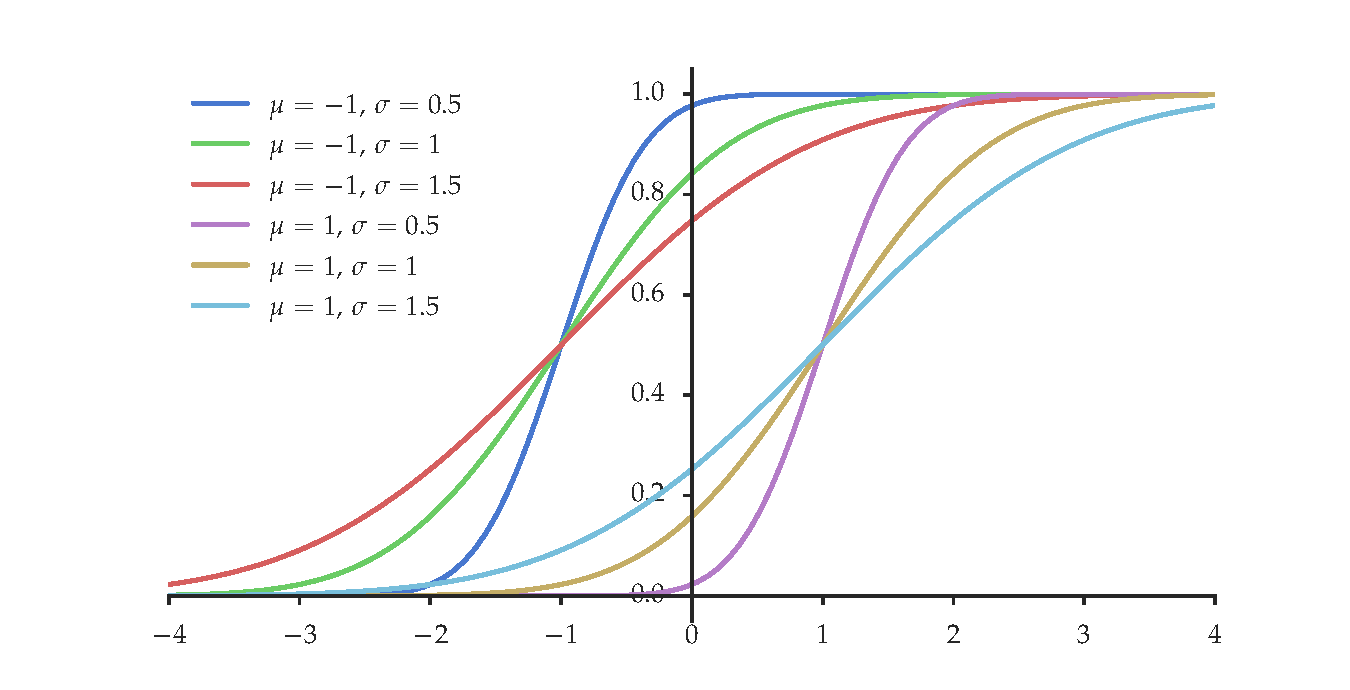
\includegraphics[trim={0 0em 0 2em}, clip]{normal_cdfs.pdf}}
    \caption{\label{f:normal_cdfs} Функция распределения для нормальных распределений }
   \end{center}
    \end{figure}
    
\end{frame}


\begin{frame}

    \vspace{2em}
    \Eg
    \navy{Распределение Парето} --- одномерное распределение
    с функция распределения вида
    %
    \begin{equation*}
        F(s) = 
        \begin{cases}
            0   
                & \text{, если } s < s_0
            \\
            1 - \left(
                    \frac{s_0}{s}
                \right)^{\alpha} 
                & \text{, если } s_0 \leq s
        \end{cases}
        \qquad (s \in \RR, \; s_0, \, \alpha > 0)
    \end{equation*}
    %
    Распределения Парето часто используются для моделирования явлений с тяжелым правым 
    хвостом, таких как распределение богатства или дохода.

\end{frame}

\begin{frame}

    \vspace{2em}
    \Eg
    Класс \navy{функции распределения бета} дан с помощью 
    %
    \begin{equation*}
        F(s) =
        \begin{cases}
            0 & \text{, если } s \leq 0
            \\
            \frac{1}{B(\alpha, \beta)}
                \int_0^s u^{\alpha-1} (1-u)^{\beta-1} \diff u
                & \text{, если } 0 < s < 1
            \\
            1   & \text{, если } 1 \leq s
        \end{cases}
    \end{equation*}
    %
   где $\alpha, \beta > 0$. 

    В этом примере $B(\alpha, \beta)$ --- \navy{функция бета} 
    %
    \begin{equation*}
        B(\alpha, \beta) 
            := \frac{\Gamma(\alpha)\Gamma(\beta)}{\Gamma(\alpha + \beta)}
        \qquad \text{where} \qquad
        \Gamma(a) := \int_0^{\infty} u^{a-1} e^{-u} \diff u
    \end{equation*}
    %
    Функция $\Gamma$ называется \navy{функция гамма}. 

\end{frame}

\begin{frame}
    
    \vspace{2em}
    \begin{figure}
       \begin{center}
        \scalebox{.45}{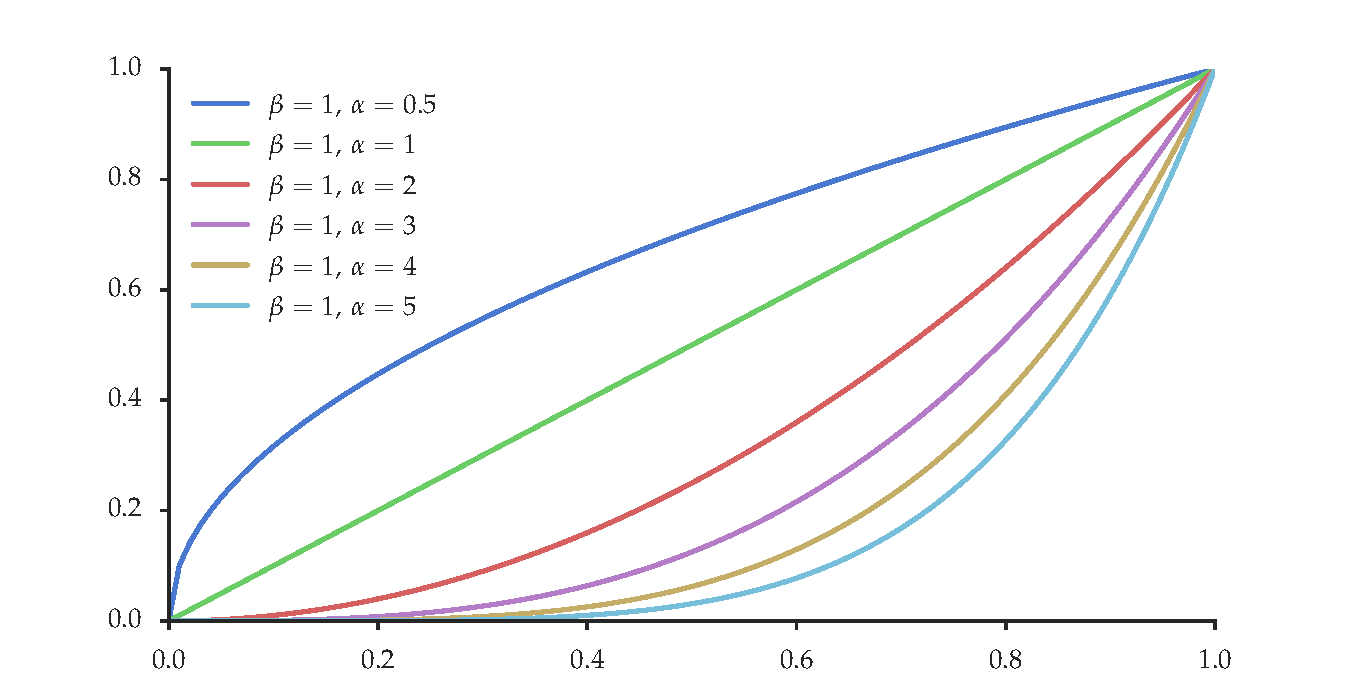
\includegraphics[trim={0 0em 0 3em}, clip]{beta_cdfs.pdf}}
        \caption{\label{f:beta_cdfs} Функции распределения бета}
       \end{center}
    \end{figure}

\end{frame}

\begin{frame}

    \Eg
    класс \navy{распределений Коши} определяется как 
    %
    \begin{equation*}
        F(s) 
        = \frac{1}{\pi} \arctan\left(  \frac{s - \tau}{\gamma} \right) 
            + \frac{1}{2}
       \qquad (s \in \RR)
    \end{equation*}
    %
    параметры $\tau \in \RR$ и $\gamma > 0$ --- параметры местоположения и масштаба 
    соответственно
    
    Если $\tau=0$ и $\gamma=1$, то $F$ называется
    \navy{стандартным распределением Коши}

\end{frame}

\begin{frame}

    \begin{figure}
       \begin{center}
        \scalebox{.45}{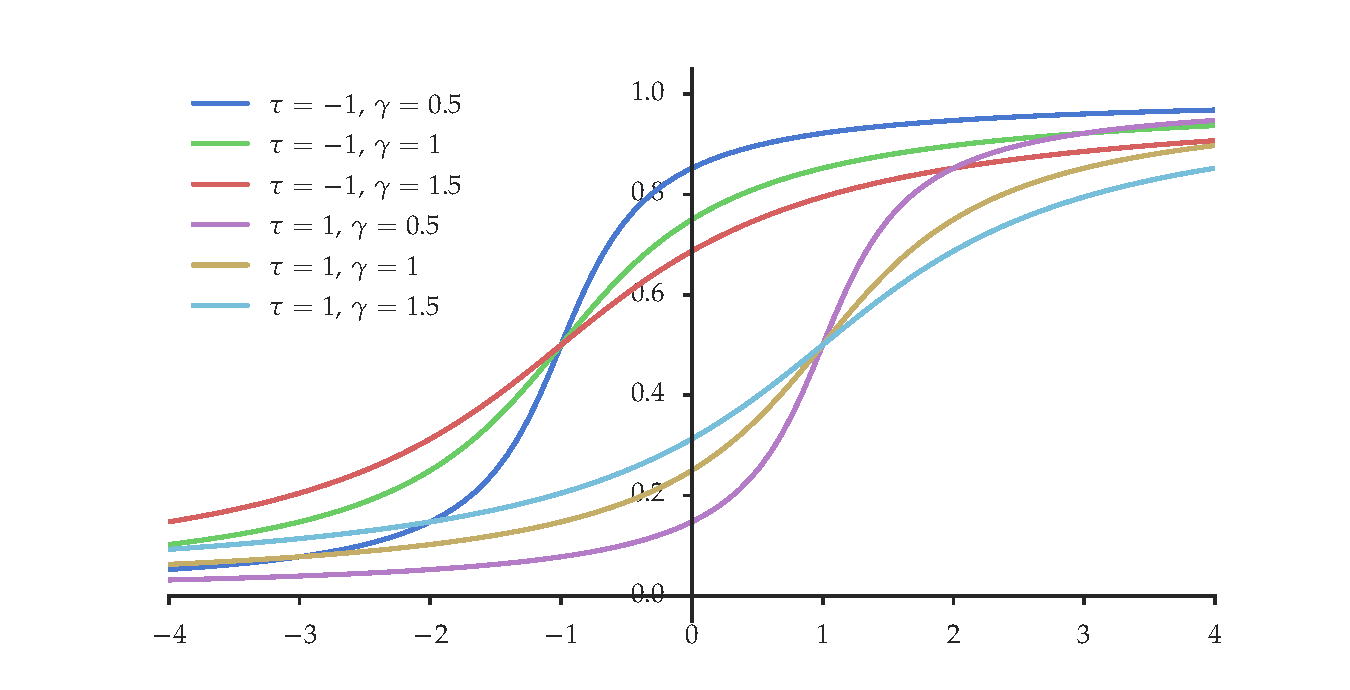
\includegraphics[trim={0 0em 0 3em}, clip]{cauchy_cdfs.pdf}}
        \caption{\label{f:cauchy_cdfs} Функции распределения Коши }
       \end{center}
    \end{figure}
    
\end{frame}

\begin{frame}

    \vspace{2em}
    \Eg
    Возьмем $a < b$, \navy{равномерная функция распределения} на промежутке $[a, b]$ --- это
    %
    \begin{equation*}
        F(s) = 
        \begin{cases}
            0 & \text{, если } s \leq a
            \\
            \frac{s-a}{b-a} & \text{, если } a < s < b
            \\
            1   & \text{, если }  b \leq s
        \end{cases}
    \end{equation*}
    %
    мы обозначаем это распределение как $U[a, b]$
        
\end{frame}

\begin{frame}

    \frametitle{Плотности и функции вероятности}

    Два удобных частных случая
    %
    \begin{itemize}
        \item дискретный: функция распределения просто скачет (ступенчатая функция) 
        \item абсолютно непрерывный случай: функция непрерывна, без скачков
    \end{itemize}

\end{frame}

\begin{frame}\frametitle{Дискретный случай}
    
    \vspace{2em}
    Распределение $P$ называется \navy{дискретным}, если оно имеет носитель распределения в счетном
    множестве; that is, если существует счетное множество $\{s_j\}_{j \geq 1}$ c
    $P(\{s_j\}_{j \geq 1}) = 1$
    
    для такого $P$ пусть
    %
    \begin{equation*}
        p_j 
        := P\{s_j\} 
        := P(\{s_j\})
        = \text{вероятность в одной точке } s_j
    \end{equation*}
    %
    \navy{Функция вероятности} --- любая неотрицательная последовательность 
    (конечная или бесконечная), сумма которой равна единице.
    
    Упражнение: покажите, что $\{p_j\}_{j \geq 1}$ является
    \navy{функцией вероятности}
    
\end{frame}

\begin{frame}

    \vspace{2em}
    Мы можем показать связь функции распределения с $P$ как:
    %
    \begin{equation}
        \label{eq:cdfdrv}
        F(s) = \sum_{j \geq 1} \1\{s_j \leq s\} p_j
    \end{equation}
    %
    так как
    %
    \begin{align*}
        F_x(s) := 
        \PP\{x \leq s\}
        & = \PP \bigcup_{j \st s_j \leq s} \{x = s_j\}
        \\
        & = \sum_{j \st s_j \leq s} \PP \{x = s_j\} 
        = \sum_{j=1}^J \1\{s_j \leq s\} p_j
    \end{align*}
    
\end{frame}

\begin{frame}

    \begin{figure}
       \begin{center}
        \begin{tikzpicture}[
    scale=5,
    axis/.style={->, >=stealth'},
    important line/.style={thick},
    dashed line/.style={dashed, thin},
    every node/.style={color=black},
    decoration={brace,amplitude=7pt},
    ]

    % define simple function
    \coordinate(O) at (0,0);
    \coordinate (s1) at (0.25,0);
    \coordinate (s2) at (0.65,0);
    \coordinate (s3) at (-0.15,0);
    \coordinate (s4) at (0.25,0.4);
    \coordinate (s5) at (0.65,0.4);
    \coordinate (s6) at (0.65,0.8);
    \coordinate (s7) at (1.1,0.8);
    % define curly bracket location
    \coordinate (c1) at (0.23,0.05); \coordinate (c2) at (0.23,0.35);
    \coordinate (c3) at (0.63,0.75); \coordinate (c4) at (0.63,0.45);
    % axis
    \draw[axis] (-0.15,0)  -- (1.1,0) node(xline)[below] {};
    \draw[axis] (0,0) -- (0,1.0) node(yline)[above] {};
    % drawing simple function
    \draw[important line,blue]  (s3) -- (s1);
    \draw[important line,blue]  (s4) -- (s5);
    \draw[important line,blue]  (s6) -- (s7);
    % dashed line
    \draw[dashed line] (s1) node[below] {$s_1$} -- (s4);
    \draw[dashed line] (s2) node[below] {$s_2$} -- (s6);
   % label y axis
   \foreach \y/\ytext in {0.8}
        \draw (0.0pt,\y cm) -- (-0.4pt,\y cm) node[anchor=east] {$1$};
   %curly bracket
   \draw [decorate,very thick] (c1) -- (c2)
   node [midway,anchor=east,inner sep=5pt, outer sep=5pt]{$p_1$};
   \draw [decorate,very thick] (c4) -- (c3)
   node [midway,anchor=east,inner sep=5pt, outer sep=5pt]{$p_2$};
   %circles
   \node[circle, draw,thin,blue,fill=white!10, scale=0.25] at (s1){};
   \node[circle, draw,thin,blue,fill=white!10, scale=0.25] at (s5){};
   \node[fill=blue,circle,scale=0.25] at (s4){};
   \node[fill=blue,circle,scale=0.25] at (s6){};
\end{tikzpicture}

        \caption{\label{f:discrete_cdf} Дискретная функция распределения}
       \end{center}
    \end{figure}

\end{frame}

\begin{frame}

    \vspace{2em}
    \Eg
    Возьмем $N \in \NN$ и $\pi \in (0, 1)$, последовательность $\{p_0, \ldots,
    p_N\}$, определяемая как
    %
    $$
        p_j = {N\choose j}\pi^j(1-\pi)^{N-j}
    $$ 
    называется \navy{биномиальной функцией вероятности}
    
    Значение $p_j$ --- вероятность, $j$ успехов в $N$ независимых
    испытаниях, вероятность успеха каждого случая равна $\pi$

\end{frame}

\begin{frame}\frametitle{Абсолютно непрерывный случай}
    
    \vspace{2em}
    \navy{Функция плотности} --- неотрицательная функция $p$ в $\RR$, которая 
    интегрируется в 1
    
    \vspace{.7em}
    Распределение $P$ \navy{определяется функцией плотности $p$}, если $p$ --- функция 
    плотности и 
    %
    \begin{equation*}
        \label{eq:drbd}
        P(B) = \int_B p(s) \diff s
        \qquad \text{для всех } B \in \bB(\RR)
    \end{equation*}
    %
    Заметим, что 
    %
    \begin{equation*}
        \int_B p(s) \diff s := \int_{-\infty}^\infty \1_B(s) p(s) \diff s
    \end{equation*}
    
\end{frame}

\begin{frame}

    \vspace{2em}
    Точное необходимое и достаточное условие существования функции плотности --- абсолютная непрерывность
    
    \vspace{.7em}
    Распределение $P$ в Борелевских подмножествах $\RR$ называется \navy{абсолютно 
    	непрерывным}, если $P(B) = 0$ всюду, где мера Лебега $B$ равна нулю 
    (смотрите \S\ref{ET-ss:measure})
    \begin{itemize}
        \item Любое счетное подмножество $\RR$ имеет меру Лебега равную нулю
    \end{itemize}
    
    \vspace{2em}
    \Fact\eqref{ET-fa:denc}
        Если $P$ абсолютно непрерывная, то $P(C) = 0$ всюду, где $C$ 
        счетно
        
\end{frame}

\begin{frame}

    \vspace{2em}
    Если распределение абсолютно непрерывно:
    
    \begin{itemize}
        \item вероятность в каждой точке равна нулю 
        \item соответствующая функция распределения не содержит скачков
        \item теорема Ньютона — Лейбница говорит, что $F(s)$
        дифференцируема во всех точках непрерывности $p$, и:
        %
        \begin{equation*}
            F'(s) = p(s)
            \qquad \text{для всех } s \in \RR \text{, таких что $p$ непрерывна в $s$}
        \end{equation*}
    \end{itemize}
    
\end{frame}

\begin{frame}

    \vspace{2em}
    \Eg
    Нормальные функции распределения дифференцируемы для всех
    $\mu$, $\sigma$, с функцией плотности
    %
    \begin{equation*}
        p(s) = F'(s) = 
        \frac{1}{\sqrt{2 \pi} \sigma}
           \exp \left\{ - 
               \frac{(s - \mu)^2}{2\sigma^2} \right\} 
    \end{equation*}
    %
    
    \vspace{.7em}
    Мы используем символ $\phi$ для стандартного нормального распределения
    
\end{frame}

\begin{frame}

    \begin{figure}
   \begin{center}
    \scalebox{.45}{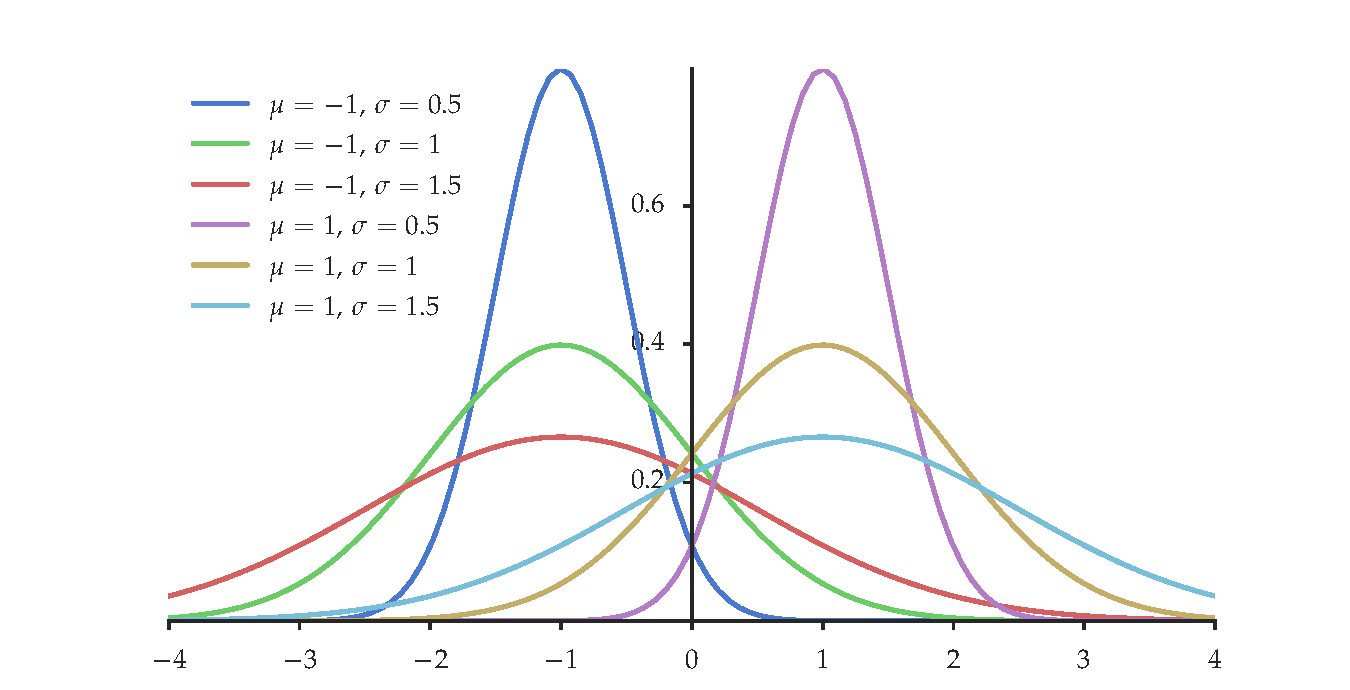
\includegraphics[trim={0 0em 0 2em}, clip]{normal_densities.pdf}}
    \caption{\label{f:normal_densities} Функции плотности нормального распределения}
   \end{center}
    \end{figure}
    
\end{frame}

\begin{frame}

    \vspace{2em}
    \Eg
    Функция распределения Коши имеет функцию плотности
    %
    \begin{equation*}
        p(s) = 
        \frac{1}{\pi \gamma}
            \left[
                1 + \left( \frac{s - \tau}{\gamma} \right)^2
            \right]^{-1}
            \qquad (s \in \RR, \; \gamma > 0, \, \tau \in \RR)
    \end{equation*}
    %
    Функции плотности Коши более остроконечны около своих мод и имеют большую массу в хвосте, чем нормальная функция плотности
    
\end{frame}

\begin{frame}

    \begin{figure}
   \begin{center}
    \scalebox{.45}{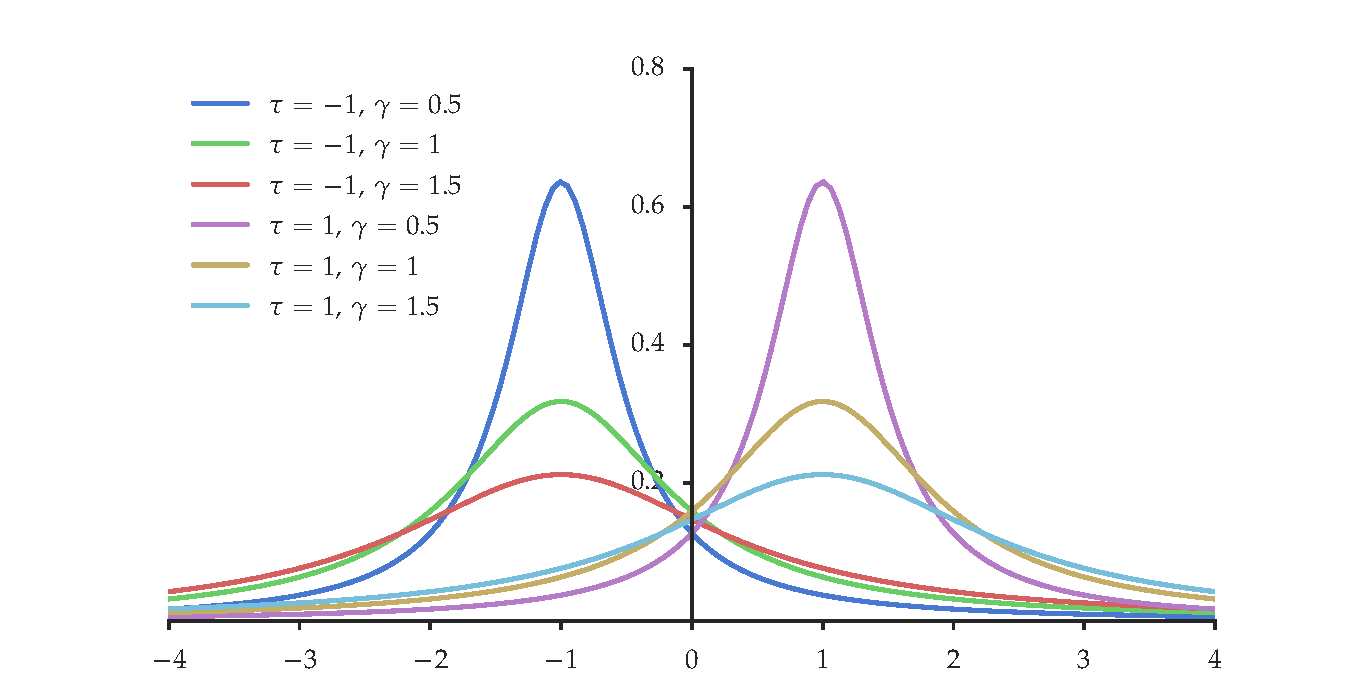
\includegraphics[trim={0 0em 0 2em}, clip]{cauchy_densities.pdf}}
    \caption{\label{f:cauchy_densities} Функции плотности Коши}
   \end{center}
    \end{figure}
    
\end{frame}

\begin{frame}

    \vspace{2em}
    \Eg
    Бета имеет функцию плотности, определяемую как
    %
    \begin{equation*}
        p(s) = \frac{s^{\alpha-1} (1-s)^{\beta-1}}{B(\alpha, \beta)}
            \qquad (\alpha, \beta > 0)
    \end{equation*}
    %
    Когда $0 < s < 1$ и $0$ в ином случае

\end{frame}


\begin{frame}

    \vspace{2em}
    \Eg
    $U[a, b]$ распределение представлено функцией плотности
    %
    \begin{equation*}
        p(s) = \frac{1}{b - a} \1\{a \leq s \leq b\}
        \qquad (s \in \RR, \; a, \, b \in \RR, \; a < b)
    \end{equation*}
    %
    
\end{frame}


\begin{frame}

    \vspace{2em}
    \Eg
    \navy{Гамма-распределение} с параметром	формы $\alpha$ и параметром
    масштаба $\beta$ --- распределение с функцей плотности
    %
    \begin{equation*}
        p(s) = 
        \frac{s^{\alpha-1} e^{-s/\beta}}{\beta^{\alpha} \Gamma(\alpha)} 
            \qquad (\alpha, \beta > 0)
    \end{equation*}
    %
    Когда $0 < s < 1$ и $0$ в ином случае
    
\end{frame}


\begin{frame}

    \vspace{2em}
    \Eg
    \navy{Хи-квадрат распределение с $k$ степенями свободы}
    --- распределение с функцией плотности
    %
    \begin{equation*}
        p(s) := \frac{1}{2^{k/2} \Gamma(k/2)} s^{k/2 - 1} e^{-s/2} 
        \qquad (s > 0,\; k \in \NN)
    \end{equation*}
    %
    Это распределение представлено символом $\chi^2(k)$
    
\end{frame}

\begin{frame}

    \begin{figure}
   \begin{center}
    \scalebox{.45}{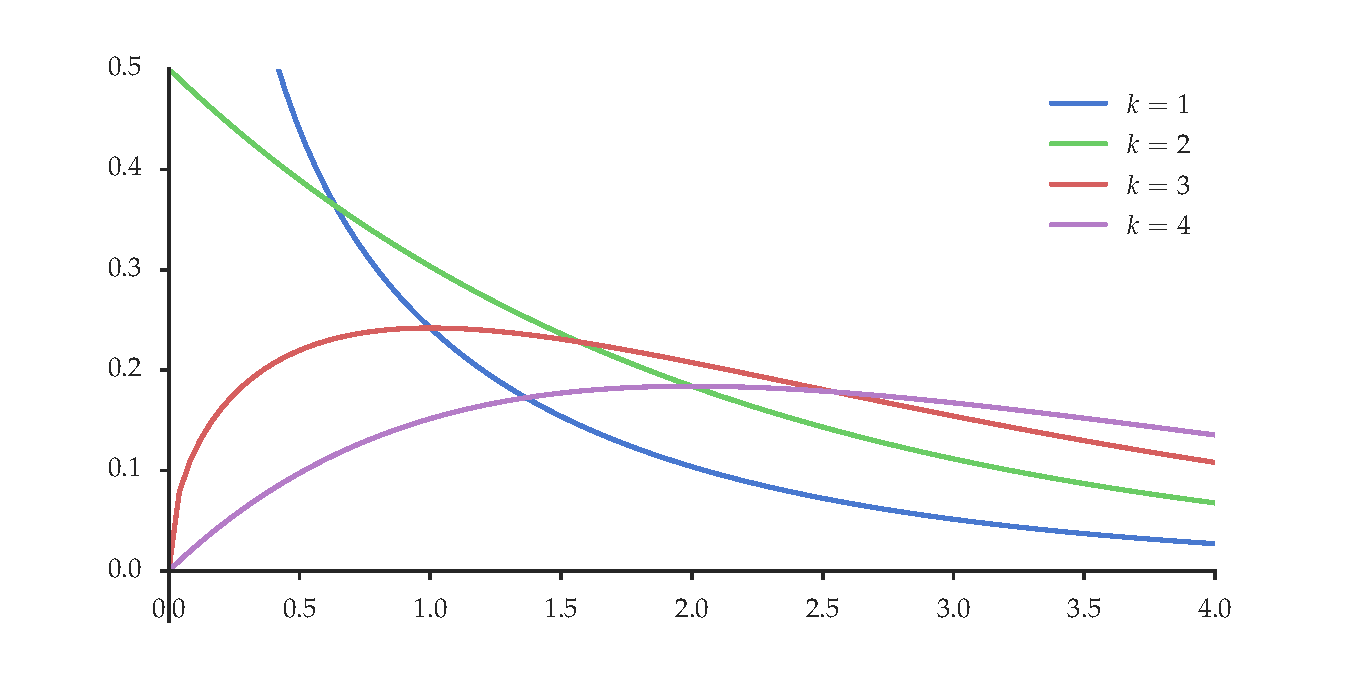
\includegraphics[trim={2em 2em 2em 2em}, clip]{chisq_densities.pdf}}
    \caption{\label{f:chisq_densities} Функции плотности хи-квадрата}
   \end{center}
    \end{figure}
    
\end{frame}

\begin{frame}

    \vspace{2em}
    \Eg
    \navy{Распределение Стьюдента $t$ с $k$ степенями свободы}, или, проще,
    $t$-распределение с $k$ степенями свободы, --- распределение в $\RR$ с
    функцией плотности
    %
    \begin{equation*}
        p(s) := \frac{\Gamma(\frac{k+1}{2})}{(k\pi)^{1/2} \Gamma(\frac{k}{2})}
        \left( 1 + \frac{s^2}{k} \right)^{-(k+1)/2}
        \qquad (s \in \RR,\; k > 0)
    \end{equation*}
    
\end{frame}

\begin{frame}

    \vspace{2em}
    \Eg
    \navy{$F$-распределение} с параметрами $k_1, k_2$ --- распределение
    с функцией плотности
    %
    \begin{equation*}
        p(s) 
        := \frac{\sqrt{(k_1 s)^{k_1}k_2^{k_2}/[k_1 s + k_2]^{k_1 + k_2}}}
            {s B(k_1/2, k_2/2)}
        \qquad (s \geq 0, \; k_1, \, k_2 > 0)
    \end{equation*}
    %
    $F$-распределение возникает при проверке ряда гипотез, как обсуждается ниже.
    
\end{frame}

\begin{frame}\frametitle{Интегрирование}

    \vspace{2em}
    Рассмотрим обычный интергал $\int_a^b
    h(s)\diff s$ функции $h$ на некотором интервале $[a, b]$
    
	Предположим, мы хотим сделать этот интергал взвешенным, придав больше массы различным частям
    $[a, b]$: $$\int_a^b h(s) p(s) \diff s$$
    
    Например:
    \begin{itemize}
        \item $h$ --- функция благосостояния и $p$ плотность агентов 
        \item $p$ --- плотность, указывающая на вероятности исходов, $h$ функция прибыли
    \end{itemize}

\end{frame}

\begin{frame}

    \vspace{2em}
	    Предположим, что $P$ не имеет функции плотности, но мы все еще хотим взвесить 
	    интеграл с помощью  $P$
    \begin{itemize}
        \item мы хотим определить $\int h(s) P(\diff s)$ 
    \end{itemize}
    
    Возьмем распределение $P$ в $\RR$ и рассмотрим $(\RR, \bB(\RR), P)$ как 
    вероятностное пространство
    
    $(\RR, \bB(\RR), P)$ имеет собственный оператор ожидания $\EEP $ 
    
    Предположим, что $h$ --- случайная величина в $(\RR, \bB(\RR), P)$, тогда
    %
    \begin{equation*}
        \EEP h :=: \int h(s) P(\diff s) 
        := \text{ожидания $h$ при $P$}
    \end{equation*}
    
\end{frame}

\begin{frame}

    \vspace{2em}
    \Fact
    Пусть $h \colon \RR \to \RR$ --- $\bB$-измерима и $P$ ---
    распределение в $\RR$
    
    Если $P$
    дискретна, с функцией вероятности $\{p_j\}_{j \geq 1}$ и носителем распределения
    $\{s_j\}_{j \geq 1}$, то
    %
    \begin{equation*}
        \label{eq:hasp}
        \int h(s) P(\diff s) = \sum_{j\geq 1} h(s_j) p_j 
    \end{equation*}
    %
    Если $P$ абсолютно непрерывно с функцией плотности $p$, то
    %
    \begin{equation*}
        \label{eq:hasd}
        \int h(s)P(\diff s) = \int_{-\infty}^{\infty} h(s) p(s) \diff s
    \end{equation*}
    %
\end{frame}


\begin{frame}\frametitle{Распределения и случайные переменные}

    \vspace{2em}
    Каждая случайная переменная 
    определяет распределение on $\RR$ 
    
    \vspace{.7em}
    Пусть $x$ --- случайная величина на некотором вероятностном пространстве $(\Omega,\fF, \PP)$:
    \begin{itemize}
        \item  вероятность $\PP\{x \in B\}$ определена
        для каждого $B \in \bB(\RR)$ (смотрите \eqref{eq:dorv})
        \item  множество функций $P$ определено как
            %
            \begin{equation}
                \label{eq:pidox}
                P(B) = \PP\{x \in B\} 
                \qquad (B \in \bB(\RR))
            \end{equation}
            %
            является \navy{распределением $x$}
    \end{itemize}
    
\end{frame}

\begin{frame}

    \vspace{2em}
     Функция распределения соответствующая распределению $P$ случайной переменной $x$ 
     удовлетворяет
    %
    \begin{equation}
        \label{eq:deffx}
        F(s) = \PP \{x \leq s\}
        \qquad (s \in \RR)
    \end{equation}
    %
    мы пишем $\lL(x) = F$, чтобы подчеркнуть, что $F$ означает распределение $x$
    
    \vspace{.7em}
    \Fact\eqref{ET-fa:axb}
    Если $\lL(x)= F$, то $\PP\{a < x \leq b\} = F(b) - F(a)$ для любых $a \leq b$
    
    Доказательство выполните в качестве упражнения (или смотрите страницу 111 в ET) 
    
\end{frame}

\begin{frame}

    \vspace{2em}
    Для каждой функции распределения $F$, существует вероятностное пространство 
    $(\Omega, \fF, \PP)$ и случайная величина $x \colon \Omega \to \RR$, 
    такая что $\lL(x) = F$;  \S\ref{ET-ss:it} показывает построение
    
\end{frame}

\begin{frame}
    
    \vspace{2em}
    Если $\lL(x) = P$ и $P$ имеет функцию плотности $p$, мы говорим, что
    \navy{$x$ имеет функцию плотности $p$}
    
    Если распределение $x$ дискретно, мы будем называть
    $x$ \navy{дискретной случайной величиной}
    
    \vspace{1em}
    \Fact
    Если $x$ имеет функцию плотности, то $\PP\{x=s\}=0$ для всех $s \in \RR$, и для
    любых $a < b$,
    %
    \begin{multline*}
        \PP\{a < x < b\}
        = \PP\{a < x \leq b\}
        \\ = \PP\{a \leq x < b\}
        = \PP\{a \leq x \leq b\}
    \end{multline*}
    %
\end{frame}

\begin{frame}\frametitle{Распределения преобразований}

    \vspace{2em}
    \Fact\eqref{ET-fa:cdftr}
    Если $\lL(x) = F$ и $y := \psi(x)$, где $\psi \colon \RR \to \RR$ 
    строго возрастает, то $\lL(y)= G$, где $G(s) := F(\psi^{-1}(s))$.
    
    \Prf
    При таких гипотезах $\psi^{-1}$ существует и
    (медленно) возрастает. Следовательно 
    %
    \begin{equation*}
        \PP\{y \leq s\} 
        = \PP\{\psi(x) \leq s\} 
        = \PP\{x \leq \psi^{-1}(s) \} 
        = F( \psi^{-1}(s) )
    \end{equation*}
    %
    Заметьте, как монотонность используется во втором равенстве

\end{frame}

\begin{frame}

    \vspace{2em}
    \Eg
    Если $\lL(x) = F$ и $y := \exp(x)$, то функция распределения $y$ --- это 
    $G(s) := F(\ln(s))$
    
\end{frame}

\begin{frame}

    \vspace{2em}
    \Fact\eqref{ET-fa:trden}
    Если $x$ имеет плотность $p$ в $\RR$ и $y := \psi(x)$, где $\psi$ ---
    диффеоморфизм в $\RR$, то распределение $y$ абсолютно
    непрерывное с функцией плотности
    %
    \begin{equation*}
        \label{eq:trden}
        q(s) = p(\psi^{-1}(s)) \left| \frac{\diff \psi^{-1}(s)}{\diff s} \right|
                 \qquad (s \in \RR)
    \end{equation*}
    
    
    \vspace{1em}
    термин \navy{диффеоморфизм} значит, что $\psi$ --- биекция в
    $\RR$ и оба $\psi$ и его обратное дифференцируемы
    
\end{frame}

\begin{frame}

    \vspace{2em}
    \Eg
    Если $x$ имеет функцию плотности $p$ в $\RR$, и $\mu$ и $\sigma$ --- константы с 
    $\sigma > 0$, то функция плотности $y := \mu + \sigma x$ --- это
    %
    \begin{equation*}
        q(s) = p \left( \frac{s - \mu}{\sigma} \right) 
                 \frac{1}{\sigma} 
                 \qquad (s \in \RR)
    \end{equation*}
    %
    Когда $x$ стандартное нормальное: $y = \mu
    + \sigma x$ is $\nN(\mu, \sigma^2)$
    
    Почему?
    \begin{itemize}
        \item Возьмем $p$ функцию плотности стандартного нормального распределения $\phi$
        \item Вспомним%
            \begin{equation*}
                p(s) = F'(s) = 
                \frac{1}{\sqrt{2 \pi} \sigma}
                   \exp \left\{ - 
                       \frac{(s - \mu)^2}{2\sigma^2} \right\} 
            \end{equation*}
    %
    \end{itemize}
    
\end{frame}

\begin{frame}

    \vspace{2em}
   Пусть $x$ --- случайная величина в вероятностном пространстве $(\Omega, \fF, \PP)$
   
   Распределение $x$ кодирует всю информацию для расчета 
   ожидания $x$ или любого $\bB$-измеримого преобразования $h(x)$
   
   Во-первых, пусть $x$ конечно. Предположим, что 
   
   \begin{itemize}
       \item  $\lL(x) = P$
       \item  функция $h\colon \RR \to \RR$ --- любая $\bB$-измеримая функция
       \item $P$ помещает все вероятности в конечное множество $\{s_j\}_{j=1}^J$
   \end{itemize}
   
   \vspace{.7em}
   Исопльзуем $\PP\{x = s_j\} = P\{s_j\}$ и определение ожиданий:
   %
    \begin{equation*}
        \label{eq:ehx}
        \EE h(x) 
        = \sum_{j=1}^J h(s_j) \PP\{x = s_j\}
        = \sum_{j=1}^J h(s_j) P\{s_j\}
        = \sum_{j=1}^J h(s_j) p_j
    \end{equation*}

\end{frame}

\begin{frame}
       
    \vspace{2em}
   Ожидания $h(x)$ в $(\Omega, \fF, \PP)$ равны
   ожиданиям $h$ в $(\RR, \bB(\RR), P)$
   
   Верно также и для бесконечного случая:
   
   \vspace{1em}
   \Fact
    Пусть $x$ --- случайная величина в некотором вероятностном пространстве $(\Omega, \fF,
    \PP)$, пусть $\lL(x) = P$ и $h$ --- $\bB$-измеримая функция, такая
    что $h(x)$ интегрируема. Ожидания $\EE h(x)$ полностью
    определены $h$ и $P$. В частности,
    %
    \begin{equation*}
        \EE h(x) = \int h(s) P(\diff s)
    \end{equation*}
    %
    где $\int h(s) P(\diff s)$ --- ожидания $h$ в $(\RR, \bB(\RR), P)$

\end{frame}

\begin{frame}

    \vspace{2em}
    \Eg
    Пусть $x$ --- случайная величина, чье распределение $P$ является равномерным
    распределением в $[a, b]$
    
    \vspace{.7em}
    Применить определение функции плотности равномерного распределения
    %
    \begin{equation*}
        \EE x 
        = \int s P(\diff s) 
        = \int s p(s) \diff s 
        = \int_{-\infty}^{\infty} 
         \frac{s}{b - a} \1\{a \leq s \leq b\} \, \diff s 
    \end{equation*}
    %
    Решение интеграла дает $\EE x = \mu := (a + b)/2$. Дисперсия равна
    %
    \begin{multline*}
        \var [x]
        = \int (s - \mu)^2 P(\diff s)
        \\ = \int_a^b
            \left(s -\frac{a + b}{2} \right)^2
            \frac{1}{b - a} \diff s
        = \frac{1}{12} (b-a)^2
    \end{multline*}
    
\end{frame}



\begin{frame}

    \vspace{2em}
    \Eg
    Предположим, что $\lL(x) = \nN(\mu, \sigma)$
    
    Если $\sigma > 0$, среднее значение может быть вычислено с помощью
    %
    \begin{equation*}
        \EE x 
        = \int_{-\infty}^{\infty} s 
        \frac{1}{\sqrt{2 \pi} \sigma}
           \exp \left\{ - 
               \frac{(s - \mu)^2}{2\sigma^2} \right\}  \diff s
        = \mu
    \end{equation*}
    %
    Дисперсия определяется как:
    %
    \begin{equation*}
        \var [x]
        = \int_{-\infty}^{\infty}
            (s - \mu)^2
            \frac{1}{\sqrt{2 \pi} \sigma}
               \exp \left\{ - 
               \frac{(s - \mu)^2}{2\sigma^2} \right\}  \diff s
        = \sigma^2
    \end{equation*}
    
\end{frame}

\begin{frame}\frametitle{Моменты распределений}

    \vspace{2em}
    Любые две случайные величины с одинаковыми распределениями
    имеют одинаковые моменты
    
    Следовательно моменты лучше всего рассматривать как
    свойство распределения, не как случайную величину
    
    \vspace{.7em}
    Таким образом, мы определяем 
    %
    \begin{itemize}
        \item \navy{среднее} $P$ как $\mu = \int s P(\diff s)$,
        \item \navy{$k$-ый момент} $P$ как $\int s^k P(\diff s)$, 
        \item \navy{дисперсию} $P$ как $\int (s - \mu)^2 P(\diff s)$,
    \end{itemize}
    %
    и так далее

\end{frame}

\begin{frame}\frametitle{Функция квантилей}

    \vspace{2em}
    Пусть $F$ --- строго возрастающая функция распределения в $\RR$
    
    Возьмем $\tau \in (0, 1)$, \navy{$\tau$-ая квантиль} $F$ --- это $\xi \in \RR$, 
    который является решением $F(\xi) = \tau$
    
    Согласно нашим предположениям о $F$, такое $\xi$ существует и однозначно определено
    
    $0.5$-ая квантиль называется \navy{медианой} $F$

\end{frame}

\begin{frame}

    \vspace{2em}
    \navy{Функция квантилей}:
    %
    \begin{equation*}
        \label{eq:quantwi}
        F^{-1}(\tau) := \text{ единственный } \xi \text{, такой что } F(\xi) = \tau
        \qquad (0 < \tau < 1)
    \end{equation*}
    
    
    \vspace{.7em}
    \Eg
    Функция квантилей связанная со стандартным распределением Коши --- это
    $F^{-1}(\tau) = \tan [\pi(\tau - 1/2)]$

\end{frame}

\begin{frame}

    \begin{figure}
   \begin{center}
    \scalebox{.44}{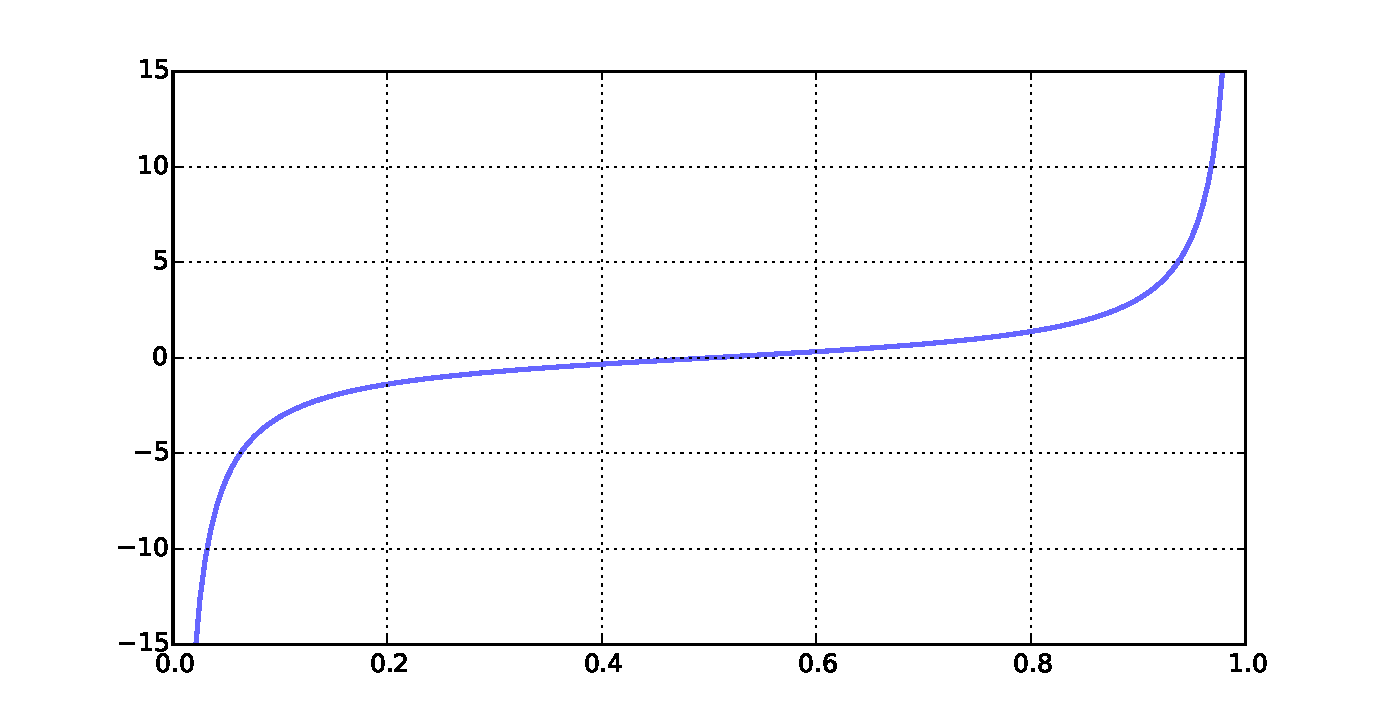
\includegraphics[trim={0 0em 0 2em}, clip]{cauchy_quant.pdf}}
    \caption{\label{f:cauchy_quant} Функция квантилей распределения Коши 
    	(горизонтальная ось --- это $\tau \in (0, 1)$)}
   \end{center}
\end{figure}

\end{frame}

\begin{frame}

    \vspace{2em}
    Когда $F$ не строго возрастающая, $F^{-1}$ не определено
    
    \vspace{1em}
    Мы можем задать:
    %
    \begin{equation}
        \label{eq:quantwi2}
        F^{-1}(\tau) := \inf \setntn{s \in \RR}{F(s) \geq \tau}
        \qquad (0 < \tau < 1)
    \end{equation}
    %
\end{frame}

\begin{frame}

    \vspace{2em}
    Функция плотности $p$ симметрична, если $p(s) = p(-s)$ для всех $s \in \RR$
    
    Распространенный сценарий проверки гипотез 
    
    \vspace{.7em}
    \Fact\eqref{ET-fa:avsc}
    Пусть $x$ --- случайная величина с функцией плотности $p$. Если $p$ симметрична, то
    функция распределения $G$ $y := |x|$ определяется как 
    %
    \begin{equation*}
        G (s) 
        := \PP\{y\leq s\} 
        = 
        \begin{cases}
            2 F(s) - 1 & \text{, если } s \geq 0
            \\
            0 & \text{ в ином случае}
        \end{cases}
    \end{equation*}
    %
    Докажите в качестве упражнения \ref{ET-ex:avsc}
    
    Факт эквивалентен $F(s) = 1 - F(-s)$

\end{frame}

\begin{frame}

    \vspace{2em}
    Возьмем случайную величину $x$ с $\lL(x) = F$ и заданной константой $\alpha \in
    (0,1)$ 
    
    \vspace{.7em}
    Рассмотрим $c$, являющийся решением $\PP\{-c \leq x \leq c \}  = 1 - \alpha$
    
    \Fact
        Если $\lL(x) = F$, $x$ имеет симметричную функцию плотности и $F$ --- строго возрастающая, то
        %
        \begin{equation}
            \label{eq:symcdf}
            c = F^{-1}(1 - \alpha/2) 
            \quad \implies \quad
            \PP\{-c \leq x \leq c\} = 1 - \alpha
        \end{equation}
        %
    Когда $F$ стандартная нормальная функция распределения $\Phi$, $c$ 
    обычно обозначается как $z_{\alpha/2}$:
    %
    \begin{equation}
        \label{eq:zalpha2}
        z_{\alpha/2} := \Phi^{-1}(1 - \alpha/2)
    \end{equation}
    
\end{frame}

\begin{frame}

    \begin{figure}
   \begin{center}
    \scalebox{.44}{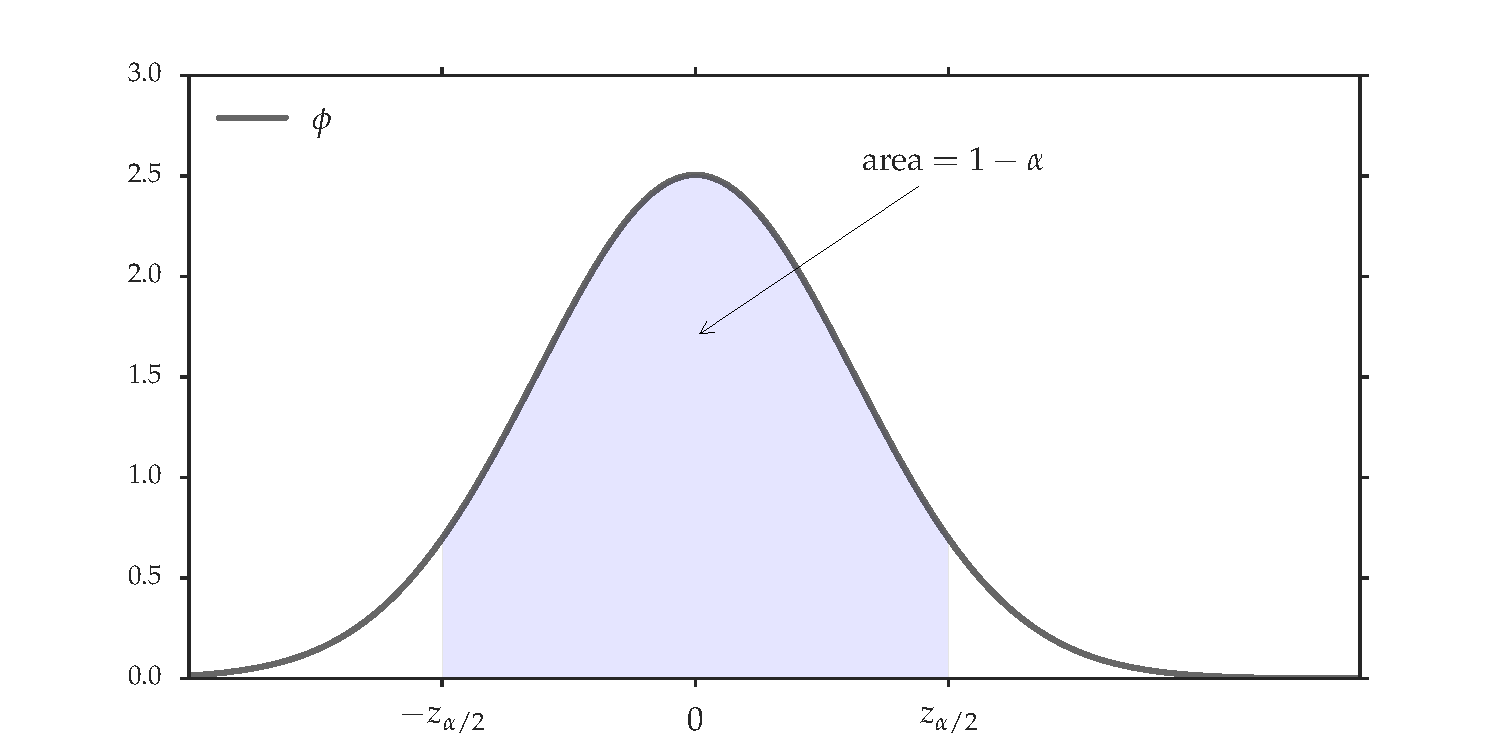
\includegraphics[trim={2em 2em 2em 2em}, clip]{fcca.pdf}}
    \caption{\label{f:fcca} Критические значения для стандартной нормальной плотности}
   \end{center}
    \end{figure}

\end{frame}


\end{document}
